\documentclass{ucrthesis-1chair}


\usepackage[mathscr]{eucal}
\usepackage{amsfonts}
\usepackage{amsmath}
\usepackage{amsthm}
\usepackage{amssymb}
\usepackage{latexsym}
\usepackage{svg}
\include{svg.dtx}
\usepackage{graphicx}
\usepackage{color}
\usepackage[noadjust]{cite}
\usepackage{epsfig}
\usepackage{tikz-cd}
\allowdisplaybreaks

\newtheorem{theoremintro}{Theorem}
\newtheorem{theorem}{Theorem}[section]
\newtheorem{proposition}[theorem]{Proposition}
\newtheorem{corollary}[theorem]{Corollary}
\newtheorem{lemma}[theorem]{Lemma}
\theoremstyle{definition}
\newtheorem{definition}[theorem]{Definition}
\newtheorem{remark}[theorem]{Remark}
\newtheorem{rmk}[theorem]{Remark}
\newtheorem{example}[theorem]{Example}
\newtheorem{conjecture}[theorem]{Conjecture}
\newtheorem{question}[theorem]{Question}

\let\nc\newcommand
\let\rnc\renewcommand
\nc{\la}{\label}
\def\bg{\begin}
\nc{\End}{{\rm{End}}}
\newcommand{\id}{{\rm{id}}}
\newcommand{\Tr}{{\rm{Tr}}}
\newcommand{\tr}{{\rm{tr}}}
\newcommand{\cl}{\mathrm{cl}}
\newcommand{\Ker}{{\rm{Ker}}}
\newcommand{\ev}{{\rm{ev}}}
\newcommand{\im}{{\rm{Im}}}
\newcommand{{\scrc}}{\mathscr{C}}
\newcommand{{\sfc}}{\mathsf{C}}
\newcommand{{\sfr}}{\mathsf{R}}
\newcommand{{\sfskein}}{\mathsf{Skein}}
\newcommand{{\sft}}{\mathsf{T}}
\newcommand{{\cs}}{\mathcal{S}}
\newcommand{{\cc}}{\mathcal{C}}
\newcommand{{\ct}}{\mathcal{T}}
\newcommand{{\ca}}{\mathcal{A}}
\newcommand{{\ck}} {\mathcal{K}}
\newcommand{{\cd}} {\mathcal{D}}
\newcommand{{\ch}} {\mathcal{H}}
\newcommand{\ci}{\mathcal{I}}
\newcommand{\xx}{{\mathbf{x}}}
\newcommand{\yy}{{\mathbf{y}}}
\newcommand{\aab}{{\mathbf{a}}}
\newcommand{\SL}{\mathrm{SL}}
\newcommand{\HH}{\mathrm{HH}}
\newcommand{\E}{\mathcal{E}}
\newcommand{\GL}{\mathrm{GL}}
\newcommand{\N}{\mathbb{N}}
\newcommand{{\Z}}{\mathbb{Z}}
\newcommand{\Q}{\mathbb{Q}}
\newcommand{\C}{\mathbb{C}}
\newcommand{\sk}{\mathrm{Sk}}
\newcommand{\fg}{\mathfrak{g}}
\newcommand{\interior}{{\rm{int}}}
\newcommand{\AP}[1]{{\color{blue} * #1}}



%%%%%%%%%%%%%%%%%%%%%%%%%%%%%%%%%%%%%%%%%%%%%%%%%%%%%%%%%%%%%%%%%%%%%%%%
% Uncomment ONE of the following two lines.  These control how the tags
% for citations are formatted (either numerical or alphabetical tag).
% Refer to the amsrefs documentation for more options.
%%%%%%%%%%%%%%%%%%%%%%%%%%%%%%%%%%%%%%%%%%%%%%%%%%%%%%%%%%%%%%%%%%%%%%%%

%\usepackage[numeric]{amsrefs}
\usepackage[alphabetic]{amsrefs}

\usepackage{microtype}				% improves spacing

%%%%%%%%%%%%%%%%%%%%%%%%%%%%%%%%%%%%%%%%%%%%%%%%%%%%%%%%%%%%%%%%%%%%%%%%
% METADATA %%%%%%%%%%%%%%%%%%%%%%%%%%%%%%%%%%%%%%%%%%%%%%%%%%%%%%%%%%%%%
%%%%%%%%%%%%%%%%%%%%%%%%%%%%%%%%%%%%%%%%%%%%%%%%%%%%%%%%%%%%%%%%%%%%%%%%

\title{***THESIS TITLE***}
\author{Alexander Pokorny}
\degreemonth{***MONTH***}			% the month name is spelled out
\degreeyear{2021}
\degreesemester{***TERM***}			% term is fall, winter, spring, etc.
\degree{Doctor of Philosophy}
\chair{Dr. Peter Samuelson}
\othermembers{%
	Dr. Jacob Greenstein \\
	Dr. Stephano Vidussi
}
\numberofmembers{2}					% number of NONCHAIR members
\field{Mathematics}
\campus{Riverside}

%%%%%%%%%%%%%%%%%%%%%%%%%%%%%%%%%%%%%%%%%%%%%%%%%%%%%%%%%%%%%%%%%%%%%%%%
% BEGIN DOCUMENT %%%%%%%%%%%%%%%%%%%%%%%%%%%%%%%%%%%%%%%%%%%%%%%%%%%%%%%
%%%%%%%%%%%%%%%%%%%%%%%%%%%%%%%%%%%%%%%%%%%%%%%%%%%%%%%%%%%%%%%%%%%%%%%%

\begin{document}

\maketitle

\copyrightpage{}

\approvalpage{}
\cleardoublepage

% FRONTMATTER %%%%%%%%%%%%%%%%%%%%%%%%%%%%%%%%%%%%%%%%%%%%%%%%%%%%%%%%%%

\begin{frontmatter}
	\setcounter{page}{4}

%%%%%%%%%%%%%%%%%%%%%%%%%%%%%%%%%%%%%%%%%%%%%%%%%%%%%%%%%%%%%%%%%%%%%%%%
% COMMENT the following two lines to omit acknowledgements.
%%%%%%%%%%%%%%%%%%%%%%%%%%%%%%%%%%%%%%%%%%%%%%%%%%%%%%%%%%%%%%%%%%%%%%%%

	\begin{acknowledgements}
	***ACKNOWLEDGEMENTS***

	This section may be omitted.
\end{acknowledgements}

	\cleardoublepage

%%%%%%%%%%%%%%%%%%%%%%%%%%%%%%%%%%%%%%%%%%%%%%%%%%%%%%%%%%%%%%%%%%%%%%%%
% COMMENT the following two lines to omit a dedication.
%%%%%%%%%%%%%%%%%%%%%%%%%%%%%%%%%%%%%%%%%%%%%%%%%%%%%%%%%%%%%%%%%%%%%%%%

	\begin{dedication}
	\null\vfill
	\begin{center}
		***DEDICATION***

		This section may be omitted.
	\end{center}
	\vfill\vfill\null
\end{dedication}

	\cleardoublepage

	\begin{abstract}
	The text of the abstract goes here.  An abstract is required, and must not exceed 350 words.  Further details can be found in UCR's formatting guidelines:

	\begin{center}
		\texttt{https://graduate.ucr.edu/document/format-guide-201920}
	\end{center}
\end{abstract}

	\cleardoublepage

	\tableofcontents
	\cleardoublepage

%%%%%%%%%%%%%%%%%%%%%%%%%%%%%%%%%%%%%%%%%%%%%%%%%%%%%%%%%%%%%%%%%%%%%%%%
% COMMENT the following two lines to omit a list of figures.  The list
% must be included if there is more than one figure.
%%%%%%%%%%%%%%%%%%%%%%%%%%%%%%%%%%%%%%%%%%%%%%%%%%%%%%%%%%%%%%%%%%%%%%%%

	\listoffigures
	\cleardoublepage

%%%%%%%%%%%%%%%%%%%%%%%%%%%%%%%%%%%%%%%%%%%%%%%%%%%%%%%%%%%%%%%%%%%%%%%%
% COMMENT the following two lines to omit a list of tables.  The list
% must be included if there is more than one table.
%%%%%%%%%%%%%%%%%%%%%%%%%%%%%%%%%%%%%%%%%%%%%%%%%%%%%%%%%%%%%%%%%%%%%%%%

	\listoftables
	\cleardoublepage

\end{frontmatter}

%%%%%%%%%%%%%%%%%%%%%%%%%%%%%%%%%%%%%%%%%%%%%%%%%%%%%%%%%%%%%%%%%%%%%%%%
% THESIS BODY %%%%%%%%%%%%%%%%%%%%%%%%%%%%%%%%%%%%%%%%%%%%%%%%%%%%%%%%%%
%%%%%%%%%%%%%%%%%%%%%%%%%%%%%%%%%%%%%%%%%%%%%%%%%%%%%%%%%%%%%%%%%%%%%%%%

\chapter{Introduction}

Summarize the main background and new results here.
\chapter{Background}


\section{Skein Theory}

\subsection{Foundations and General Notions}
In this work, we will be forced to discuss a few different variants of skein modules. For this reason, it will be useful to first describe some general framework of skein theory so that each of these variants will be a special case. Unless otherwise stated, we will assume $M$ is an oriented $3$-manifold with boundary $\partial M$ (possibly empty), $\Sigma$ is an oriented surface, $I$ is the real interval $[0,1]$, $R$ is a commutative and unital ring. 

\begin{definition}
    Let $T_1, T_2: X \to M$ be smooth embeddings of a smooth manifold $X$ into $M$. A \textbf{smooth ambient isotopy} $H: T_1 \Rightarrow T_2$ is a smooth homotopy of diffeomorphisms $H_t: M \to M$ such that $H_0=\id_M$ and $H_1 \circ T_1 = T_2$. Furthermore, we demand that the boundary $\partial M$ is fixed by the homotopy. 
\end{definition}

The relation 
\[
T_1 \sim T_2 \textrm{ if and only if there exists a smooth ambient isotopy } H: T_1 \Rightarrow T_2
\]
is an equivalence relation. The smoothness requirement of $H$ is important when considering knots. Without it, all knots would be equivalent to the unknot by contracting all of the complexity of the knot to a point. 

\begin{definition}
Let $N$ be a finite set of points contained in the boundary $\partial M$. An \textbf{$N$-tangle} in $M$ (or just \textit{tangle} for short) is the smooth ambient isotopy class of a smooth embedding 
\[
T: \underbrace{\underset{j \in J}{\bigsqcup}\, S^1}_{:=L} \sqcup \underbrace{\underset{k \in K}{\bigsqcup}\, I}_{:=B} \to M
\]
for some finite sets $J$ and $K$ such that
\begin{enumerate}
\item the image of $L$ lies in the interior of $M$,
\item the image of the interior of $B$ lies in the interior of $M$,
\item the image of the boundary of $B$ equals $N$.
\end{enumerate}
If $B$ is empty, then the result is called a \textbf{link} in $M$. Similarly, if $L$ is empty, then it's called a \textbf{braid} in $M$. 

One may also consider \textit{oriented} or \textit{framed} tangles by choosing an orientation or framing for each point in $N$ and for each connected component of $L$ and $B$ such that the choices are compatible with each other with respect to the smooth embedding.
%For our purposes, the difference between framed and unframed tangles will be a matter of convention; we choose to work with framed tangles as is standard in the literature. 
If $M = \Sigma \times I$, then we will assume that the points in $N$ are contained in $\Sigma \times \{ \frac{1}{2} \}$ and that their framings are thought to be embedded orthogonally to $\Sigma \times \{ \ast \}$. 
\end{definition}

We say a framed tangle in $\Sigma \times I$ has \textbf{blackboard framing} if the entire framing is embedded orthogonally to $\Sigma$. Every framed link in $\Sigma \times I$ is isotopic to one with a blackboard framing by turning each twist into a loop with a local blackboard framing:

\[
    \vcenter{\hbox{\includegraphics[height=3cm]{twist.eps}}} \quad = \quad \vcenter{\hbox{\includegraphics[height=3cm]{invvh2.eps}}}.
\]
This suggests that we may represent framed links in $\Sigma \times I$ as link diagrams on $\Sigma$. Indeed, equivalence under ambient isotopy is captured by the Reidemeister moves 2, 3, and a modified Reidemeister move 1:

\[
    \vcenter{\hbox{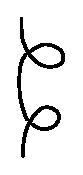
\includegraphics[height=3cm]{modifiedr1.eps}}} \quad = \quad \vcenter{\hbox{
\includegraphics[height=3cm]{modifiedr1resolution.eps}}}.
\]

\AP{Add pictures of RII and RIII for good measure.}
Below are some examples of framed tangle diagrams.

\[
    \vcenter{\hbox{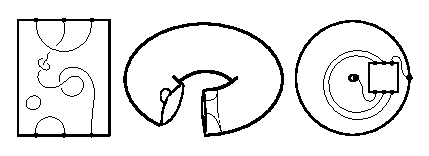
\includegraphics[height=3cm]{Ntangles.eps}}}
\]

Define the \textbf{writhe} of a tangle diagram is the number of positive crossings minus the number of negative crossings. It is easy to see that the Reidemeister moves above preserve the writhe of a diagram, so the concept is well defined. Writhe should be thought of as a grading on the free $R$-module on the set of tangles in the given space, which provides a good reason to work with framed links over ordinary links. Such a module is a main ingredient of this theory, so let's honor it with a proper discussion.

\begin{definition}
Let $\ct(M, N)$ be the free $R$-module generated by the set of framed $N$-tangles in $M$. Analagously, we can define $\ct^{or}(M,N)$ to be the free $R$-module generated by the set of oriented framed $N$-tangles in $M$. All definitions which are to follow in this subsection have an analagous definition using oriented tangles. Also, we will formally define $\cs_R(\varnothing, \varnothing) := R$. 
\end{definition}

The construction $\ct( -, -)$ is actually a symmetric monoidal functor $\ct: \sfc \to R\textsf{-Mod}$ for a careful choice of category $\sfc$ which we now describe. The objects of $\sfc$ are pairs $(M, N)$ of the same type as discussed previously. A morphism $(f, W): (M', N') \to (M, N)$ is a pair of a smooth, orientation-preserving embedding $f: M' \to M$ such that $M - f(M')$ is either a smooth 3-manifold or the empty set, and choice of $W \in \ct\big( M-f(M'), N \sqcup f(N') \big)$ (unless $M - f(M')$ is empty, in which case $W$ is a formal symbol for the "empty link" in the empty set). Composition is given by $(g, W') \circ (f, W) = (g \circ f, W' \cup W)$, which is associative since $\circ$ and $\cup$ are associative.

\AP{Give a picture of composition in $\sfc$.}

The induced map denoted $W: \ct(M', N') \to \ct(M, N)$ is a linear map defined by $W(T) = W \cup T$, and we will refer to such a linear map $W$ as a \textbf{wiring}. We are abusing notation by denoting this linear map by $W$, but it should be clear from the context what $f$ is since it is technically encoded in the data of the element $W \in \ct\big( M-f(M'), N \sqcup f(N') \big)$. It is true that $\ct$ preserves composition and identity morphisms, making and so $\ct$ is functorial. $\sfc$ can now be equipped with a symmetric monoidal structure via disjoint union. It is clear that 
\[\cs_R(M \sqcup M', N \sqcup N') \cong \cs_R(M, N) \underset{R}{\otimes} \cs_R(M', N')\]
for any sets of framed points $N \subset \partial M$ and $N' \subset \partial M'$. The unit is given by the object $(\varnothing, \varnothing) \in \sfc$ and define $\ct(\varnothing, \varnothing) := R$, which makes $\ct$ a symmetric monoidal functor. 

\begin{definition}
Let $B$ be the smooth closed $3$-ball, $N_i$ be some collection of $2i$ boundary points of $B$, and let $X \subset \underset{i \in \N}{\bigsqcup} \ct(B, N_B)$ be some (typically finite) set, which we will call a set of \textbf{skein relations}. Given any tangle module $\ct(M, N_M)$, there exists a submodule $\ci(X)$ generated by the set 
\[\{ W(x) \mid x \in X \text{ and } W:\ct(B, N_B) \to \ct(M, N_M) \text{ is a wiring diagram} \}.\] 
A quotient of the form $\cs_X(M, N) := \ct(M, N) / \ci(X)$ is called a \textbf{skein module} of $M$ relative to $N$. If $N = \varnothing$ is the empty set, we may use the notation $\cs_X(M) := \cs_X(M, \varnothing)$. Similar definitions may be given using oriented and/or unframed tangles instead. 
\end{definition}
The construction $\cs_X(-, -)$ is a functor in the same way that $\ct(-, -)$ is; a smooth, orientation-preserving embedding $f: M \to M'$ and an element $W \in \cs_X\big( M-f(M'), N \sqcup f(N') \big)$ defines a linear map $W: \cs_X(M, N) \to \cs_X(M', N')$. In fact, the quotient maps $\alpha_{(M, N)}: \ct(M, N) \to \cs_X(M, N)$ yield a natural transformation. In other words, given a morphism $(M, N) \to (M', N')$ in $\sfc$, the diagram
\begin{center}
\begin{tikzcd}
	\ct(M, N) \arrow[d,"\alpha_{(M, N)}"] \arrow[r, "W"] 
	& \ct(M', N') \arrow[d, "\alpha_{(M', N')}"]\\
	\cs_X(M, N) \arrow[r, "W"] & \cs_X(M', N')
\end{tikzcd}
\end{center}
commutes. Such a functor will be called a $\textbf{skein theory}$. 

For any oriented surface $\Sigma$, we can define a category $\sfskein_X(\Sigma)$ which we will call a $\textbf{skein category}$. The objects of this category are finite sets of framed points $N$ in $\Sigma$, and the morphisms $N \to N'$ are elements of $\cs_X\big(\Sigma \times I, (N \times \{0\}) \sqcup (N' \times \{1\})\big)$, so the category is $R$-linear. Write composition of morphisms by concatenation. If $y:N \to N'$ and $z:N' \to N''$ are morphisms, then their composite $yz:N \to N''$ is constucted by gluing $z$ on $y$ through $N'$ and rescaling the interval coordinate appropriately.

\AP{Picture of composition in $\sfskein_X(\Sigma)$.}

The endomorphism algebras in this category are called \textbf{skein algebras} and are denoted by $\cs_X(\Sigma, N) := \cs_X(\Sigma \times I, (N \times \{0\}) \sqcup (N \times \{1\}) \big)$. If $N$ is the empty set, then we reduce the notation to simply $\cs_X(\Sigma)$.

If $f: \Sigma \to \Sigma'$ is a smooth embedding of surfaces, then there is an induced functor 
\[
\sfskein_X(f): \sfskein_X(\Sigma') \to \sfskein_X(\Sigma)
\]
defined on objects by $\sfskein_X(f)(N) = f(N)$ and on morphisms in the following way. First, extend $f$ trivially to $f \times \id_I: \Sigma \times I \to \Sigma' \times I$. Then, in the skein algebra of the complement of the image of $f \times \id_I$, choose the multiplicative identity element $e \in \cs_X\big( \Sigma' - \im(f) \big)$ which is the empty tangle. The pair $(f \times \id_I, e)$ is an object in the category $\sfc$, which gives rise to a wiring
\[e: \cs_X\Big(\Sigma \times I, \big(N \times \{0\}\big) \sqcup \big(N' \times \{1\}\big) \Big) \to \cs_X\Big(\Sigma' \times I, \big(f(N) \times \{0\}\big) \sqcup \big( f(N') \times \{1\} \big) \Big)\]
via the functor $\cs_X$. Now we may define what $\sfskein_X(f)$ does to morphisms: $\sfskein_X(f)(y) = e(y)$ for any $y \in \cs_X\Big(\Sigma \times I, (N \times \{0\}) \sqcup (N' \times \{1\}) \Big)$.

\AP{Picture of how $\sfskein_X(f)$ works on morphisms.}

It is clear that $\sfskein_X(f)$ preserves composition and identity morphisms. Therefore, if we let $\mathsf{Surf}$ be the category of smooth embeddings between smooth oriented surfaces, we can summarize our last few points by saying we have a functor
\[
\sfskein_X: \mathsf{Surf} \to \mathsf{Cat}.
\]
In particular, $\sfskein_X(f)$ defines algebra homomorphisms on the skein algebras
\[e: \cs_X\big(\Sigma, N\big) \to \cs_X\big(\Sigma', f(N)\big).\]
\AP{We use this type of algebra homomorphism when we embed the annulus into the torus.}

The above homomorphisms are a special case of a more general type of map. If $N$ is a set of framed points on $\Sigma$, then a smooth embedding $f: \Sigma \to \partial M$ induces a $\cs_X(\Sigma, N)$-module structure on $\cs_X\big(M, N'\big)$ for any $N'$ with $f(N) \subseteq N'$. The action is given by ``pushing tangles in through the boundary". In other words, the pre-composition of a smooth embedding of a collar neighborhood $g: \partial M \times I \to M$ with $f \times \id_I: \Sigma\times I \to \partial M \times I$ induces a bilinear map
\[
\cs_X(\Sigma, N) \times \cs_X(M, N') \to \cs_X(M, N')
\]
because $M$ minus a collar neighborhood is diffeomorphic to itself. Alternatively, a choice of element in $\cs_X(\Sigma, N')$ produces a wiring $\cs_X(M, N') \to \cs_X(M, N')$.

\AP{Picture of action.}

\subsection{Examples of Skein Theories}

The last subsection leaves us with an important and unanswered question. Which sets of skein relations $X$ produce interesting skein theories? One class of examples is found by examing sets of relations satisfied by morphisms in a linear ribbon category. Ribbon categories are braided monoidal categories which are rigid and equipped with a twist morphism for every object, satisfying some compatibility conditions. The axioms are such that the morphisms may be interpreted as framed braid diagrams. In particular, the morphisms satisfy the Reidemeister moves shown previously. We will discuss three examples of skein theories derived from skein relations which are meant to emulate linear relations satisfied by the braid and twist morphisms in certain ribbon categories coming from the representation theory of quantum groups, a topic which has generated a lot of interest from mathematicians since the 1980s. Quantum groups provided a class of non-commutative and non-cocommutative Hopf algebras which are not constructed in a trivial way (such as taking a tensor product of one non-commutative and one non-cocommutative Hopf algebra). Furthermore, the categories of representations of quantum groups are braided monoidal categories with non-involutive braidings. The skein relations below capture how far off the braidings are from being involutive.  

Here, we are forced to fix a base ring. For our purposes, $R$ must be a commutative ring containing invertible elements $s$ and $v$. Typical choices of $R$ are $\Z[s^{\pm 1}, v^{\pm 1}], \Q(s, v)$, or some other ring in between these.  In particular, the theorem \AP{Cite BB} is stated over this ring, a result we will depend heavily on later on. \\

\begin{example}[\textit{Kauffman (Dubrovnik) Skein Relations}]
Let $X_1$ denote the set of two unoriented skein relations
\begin{flalign*}
    \vcenter{\hbox{\includegraphics{poscross.eps}}} &= \vcenter{\hbox{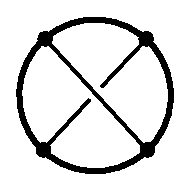
\includegraphics{negcross.eps}}} + (s-s^{-1}) \,\, \vcenter{\hbox{\includegraphics{idresolution.eps}}} - (s-s^{-1}) \,\, \vcenter{\hbox{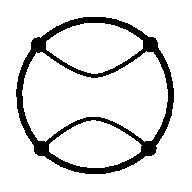
\includegraphics{capcupresolution.eps}}} \\ \\
    \vcenter{\hbox{\includegraphics{vh.eps}}} &= v \,\, \vcenter{\hbox{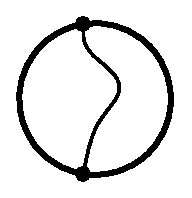
\includegraphics{frameresolution.eps}}}.
\end{flalign*}
The functor $\cd(-,-) := \cs_{X_1}(-,-)$ is the Dubrovnik skein theory (sometimes just called the Kauffman skein theory). We will use the notation $\mathsf{D} := \sfskein_{X_1}$ for the Dubrovnik skein categories. Using the Dubrovnik variant is important for us (see \AP{universal enveloping algebra result}). This theory is related to Dubrovnik polynomials in that the Dubrovnik polynomial of a link is a normalized value of the link in $\cd(S^3)$. The normalization is often so that the Dubrovnik polynomial of the unknot is $1$, whereas the value of the unknot in $\cd(S^3)$ is $\delta_\cd := 1 - \frac{v-v^{-1}}{s-s^{-1}}$, which can be deduced from the skein relations.
\end{example}

\begin{example}[\textit{HOMFLYPT Skein Relations}]
Next, let $X_2$ denote the set of two oriented skein relations
\begin{flalign*}
    \vcenter{\hbox{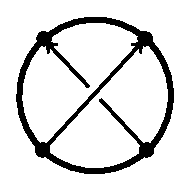
\includegraphics{poscrossor.eps}}} &= \vcenter{\hbox{\includegraphics{negcrossor.eps}}} + (s-s^{-1}) \,\, \vcenter{\hbox{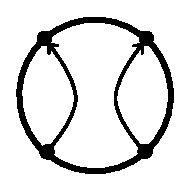
\includegraphics{idresolutionor.eps}}} \\ \\
    \vcenter{\hbox{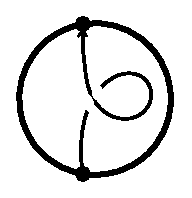
\includegraphics{vhor.eps}}} &= v \,\, \vcenter{\hbox{\includegraphics{frameresolutionor.eps}}}
\end{flalign*}
The functor $\ch(-,-) := \cs_{X_2}(-,-)$ is the HOMFLYPT skein theory and we use the notation $\mathsf{H} := \sfskein_{X_2}$ for the HOMFLYPT skein categories. As in the Dubrovnik case, this theory is related to HOMFLYPT polynomials so that the HOMFLYPT polynomial of a link is a normalized value of the link in $\ch(S^3)$. Again, some often make the choice to normalize this polynomial so that the value of the unknot is $1$, but the value of the unknot in $\ch(S^3)$ is $\delta_\ch := -\frac{v-v^{-1}}{s-s^{-1}}$.
\end{example}

\begin{example}[\textit{Kauffman Bracket Skein Relations}]
As a final example, let $X_3$ denote the set of two unoriented skein relations
\begin{flalign*}
    \vcenter{\hbox{\includegraphics{poscross.eps}}} &= s \,\, \vcenter{\hbox{\includegraphics{idresolution.eps}}} + s^{-1} \,\, \vcenter{\hbox{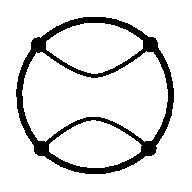
\includegraphics{capcupresolution.eps}}} \\ \\
    \vcenter{\hbox{\includegraphics{vh.eps}}} &= -s^{-3} \,\, \vcenter{\hbox{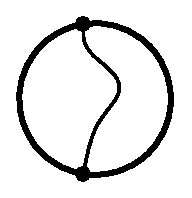
\includegraphics{frameresolution.eps}}}
\end{flalign*}
The functor $\ck(-,-) := \cs_{X_3}(-,-)$ is the Kauffman bracket skein theory (not be confused with the Kauffman skein theory) and we use $\mathsf{K} := \sfskein_{X_3}$ to notate the Kauffman bracket skein categories. The value of a link in $\ck(S^3)$ is equal to its bracket polynomial, which may be normalized as above to obtain its Jones polynomial. 
\end{example}

\begin{remark}
Any linear combination of tangles which satisfy the Dubrovnik skein relations will also satisfy the Kauffman bracket skein relations after making the specialization $v=-s^{-3}$. Therefore, there is a natural transformation of skein theories $\cd(-,-) \to \ck(-,-)$ induced by the intentity map on link diagrams. 
\end{remark}

In this work, we will focus more on the Dubrovnik and the HOMFLYPT skein theories, but will make a few mentions regarding the Kauffman bracket skein theory when it is valuable for us to do so. It is worth mentioning that many of the theorems and proofs relating to the Dubrovnik and HOMFLYPT skein theories have been insipired by analagous work about the Kauffman bracket skein theory. 

\subsection{Skein algebras of tangles in a cube}

In the case where $\Sigma = I \times I$, the endomorphism objects of $\mathsf{D}(\Sigma), \mathsf{H}(\Sigma)$, and $\mathsf{K}(\Sigma)$ are known and provide the motivation for why the choices of skein relations are what they are. For an integer $n \geq 1$, let $[n]$ be a set of $n$ points in $\Sigma$, chosen to be evenly spaced along the line segment $\frac{1}{2} \times I$. Then the endomorphism algebras 
\[
BMW_n := \End_\mathsf{D}(\Sigma)([n]), \qquad H_n := \End_\mathsf{H}(\Sigma)([n]), \qquad TL_n := \End_\mathsf{K}(\Sigma)([n])
\]
are known to be isomorphic to the Birman-Murakami-Wenzl, (Type A) Hecke, and Temperley-Lieb algebras, respectively (\AP{*Add citations}). 

Let $q \in \C$ be not a root of unity, $U_q(\mathfrak{gl}_N)$ be the Drinfeld-Jimbo quantum group associated to the Lie algebra $\mathfrak{gl}_N$, and $V$ be the natural representation of $U_q(\mathfrak{gl}_N)$ (\AP{cite CP}). Then $H_n$ acts on the $n$-fold tensor product $V^{\otimes n}$ by $U_q(\mathfrak{gl}_N)$-linear endomorphisms, and this action generates $\End_{U_q(\mathfrak{gl}_N)}(V^{\otimes n})$. This is actually part of the statement of quantum Frobenius-Schur-Weyl duality: $V^{\otimes n}$ is a $U_q(\mathfrak{gl}_N)$-$H_n$-bimodule, and the action of one algebra generates the linear endomorphisms with respect to the other. So a representation of one algebra determines a representation of the other via tensor product with $V^{\otimes n}$. The Birman-Murakami-Wenzl algebra plays the role of the Hecke algebra for $U_q(\mathfrak{g}_N)$ in the case where $\mathfrak{g}$ is one of the orthogonal or symplectic Lie algebras. For this reason, from a Lie theoretic point of view, the HOMFLYPT skein theory is thought of as a ``type A" theory, while the Dubrovnik skein theory is a ``types B, C, D" skein theory.

As for the Temperley-Lieb algebra $TL_n$, it acts on the $n$-fold tensor power $V^{\otimes n}$ of the natural representation of $U_q(\mathfrak{gl}_2)$. Actually, there is a surjective algebra homomorphism $H_n \to TL_n$ and the action $H_n \to \End_{U_q(\mathfrak{gl}_2)}(V^{\otimes n})$ factors through this homomorphism. One can conclude that the action of $H_n$ on $V^{\otimes n}$ is not faithful, at least in the case when $N=2$ and $n \geq 1$.


\subsection{Skein algebras of the annulus}

\subsection{HOMFLYPT and Kauffman Skein Modules}

\subsection{The Iwahori-Hecke Algebra and the BMW Algebra}

\subsection{Skein Algebras of the Annulus}

\subsection{Connections to Representation Theory}

\subsection{A Relative Skein Algebra of the Annulus}

\subsection{The HOMFLYPT Skein Algebra of the Torus}



\section{The Ring of Symmetric Functions}

\subsection{Character Rings of Classical Groups}

\subsection{Bases of $\Lambda$ and Identities}
\chapter{The Skein Algebra of the Torus}

\AP{Add some introduction and remark about collaboration.}


\section{Power Sum Elements}

Recall that there is a injective algebra homomorphism $\Lambda \to \ch(A)^+$ which sends the Schur function $s_\lambda$ to the minimal idempotent closure $Q_\lambda$. Use $h_n := Q_{(n)}$ to denote the image of the $n^\textrm{th}$ complete homogeneous symmetric function under this homomorphism. In \AP{MS} the authors import power sum elements from $\Lambda$ to $P_k \in \ch(A)$. The power sum elements have a concrete definition in $\Lambda$, but alternatively they may be defined using an equation of formal power series in the ring $\ch(A)[[t]]$ as
\begin{equation}
\sum_{k=1}^\infty \frac{P_k}{k} t^k = \ln \Bigg( 1 + \sum_{n=1}^\infty h_n t^n \Bigg)
\end{equation}
which writes each $P_k$ in terms of the generators $h_n$. 

Using the Beliakova-Blanchet section $\Gamma: H_n \to BMW_n$, we may emulate this definition to define ``power sum" elements $\tilde{P}_k \in \cd(A)$ by the formal power series equation
\begin{equation}
\sum_{k=1}^\infty \frac{\tilde{P}_k}{k} t^k = \ln \Bigg( 1 + \sum_{n=1}^\infty \tilde{h}_n t^n \Bigg)
\end{equation}
where $\tilde{h}_n := \tilde{Q}_{(n)}$ is the annular closure of the BMW symmetrizers $\tilde{y}_n = \Gamma(y_n)$.

Let's now continue our discussion of Section \ref{sec:relativeannulus} with the following theorem.

\begin{theorem} \label{thm:powersumcommutator}
For any $k \geq 1$, the relation
\begin{equation} \label{eq:powersumcommutator}
e \cdot \tilde{P}_k - \tilde{P}_k \cdot e = (s^k - s^{-k}) (a^k - a^{-k})
\end{equation}
holds. Equivalently,
\begin{equation}
a^i \cdot \tilde{P}_k - \tilde{P}_k \cdot a^i = (s^k - s^{-k}) (a^{k+i} - a^{-k+i})
\end{equation}
for any integer $i$.
\end{theorem}

We will split the proof of this theorem into two technical lemmas.

\begin{lemma} \label{lem:powersumcommutator1}
The relations of Theorem \ref{thm:powersumcommutator} hold if and only if 
\begin{equation} \label{eq:skewcommutator}
e \cdot (\tilde{h}_{n+2} + \tilde{h}_n) - (\tilde{h}_{n+2} + \tilde{h}_n) \cdot e = (sa + s^{-1}a^{-1}) (e \cdot \tilde{h}_{n+1}) - (s^{-1}a + sa^{-1}) (\tilde{h}_{n+1} \cdot e)
\end{equation}
for all integers $n \geq -1$, where $\tilde{h}_0 := 1$ and $\tilde{h}_{-1} := 0$.
\end{lemma}
\begin{proof}
The relations of Theorem \ref{thm:powersumcommutator} may be organized into a single power series equation
\begin{equation} \label{eq:skewcommutator}
\sum_{k=1}^\infty \frac{e \cdot \tilde{P}_k - \tilde{P}_k \cdot e}{k} t^k = \sum_{k=1}^{\infty} \frac {(s^k - s^{-k}) (a^k - a^{-k})}{k} t^k
\end{equation}
in $\ca_\cd [[t]]$. Rewrite this equation as
\begin{equation} \label{eq:powersumcommutator2} 
e \cdot \Bigg( \sum_{k=1}^\infty \tilde{P}_k \Bigg) - \Bigg( \sum_{k=1}^\infty \tilde{P}_k \Bigg) \cdot e = \sum_{k=1}^{\infty} \frac {(sat)^k}{k} + \sum_{k=1}^{\infty} \frac {(s^{-1}a^{-1}t)^k}{k} - \sum_{k=1}^{\infty} \frac {(s^{-1}at)^k}{k} - \sum_{k=1}^{\infty} \frac {(sa^{-1}t)^k}{k}
\end{equation}
We can make sense of the left-hand side by extending the algebra homomorphism $x \mapsto e \cdot (x)$ to an algebra homomorphism of rings of formal power series
\begin{center}
\begin{tikzcd}
\cd(A) \arrow[r, "e \cdot (-)"] \arrow[d, hook] & \ca_\cd \arrow[d, hook] \\
\cd(A)[[t]] \arrow[r, "e \cdot (-)"] & \ca_\cd[[t]]
\end{tikzcd}
\end{center}
and similarly for $(-) \cdot e$. Now for shorthand, define 
\[
H(t) := 1 + \sum_{n=1}^\infty \tilde{h}_n t^n
\]
and recall the Taylor series expansion
\[
-\ln(1-x) = \sum_{k=1}^\infty \frac{x^k}{k}
\]
which is a variation of the Newton-Mercator series. Then the Equation \eqref{eq:skewcommutator} becomes
\begin{equation} \label{eq:powersumcommutator3} 
e \cdot \Big( \ln\big(H(t)\big) \Big) - \Big( \ln \big(H(t)\big) \Big) \cdot e = - \ln(1 - sat) - \ln(1 - s^{-1}a^{-1}t) + \ln(1 - s^{-1}at) + \ln(1 - sa^{-1}t).
\end{equation}
The maps $e \cdot (-)$ and $(-) \cdot e$ commute with the natural logarithm. Use this and other natural log properties to write
\begin{equation}
\ln\Big( e \cdot \big( H(t) \big) \big( 1 - (sa + s^{-1}a^{-1})t + t^2 \big) \Big) = \ln\Big( \big( H(t) \big) \cdot e \big( 1 - (s^{-1}a + sa^{-1})t + t^2 \big) \Big).
\end{equation}
Exponentiating both sides and equating coefficients gives the system of equations defined in the statement of the lemma. Each step of the proof is invertible, and thus the two sets of relations are logically equivalent.
\end{proof}

\begin{lemma}
The relations of Lemma \ref{lem:powersumcommutator1} hold.
\end{lemma}
\begin{proof}
If $n=-1$, the relation we would like to show becomes 
\begin{equation*}
e \cdot \tilde{h}_1 - \tilde{h}_1 \cdot e = \{1\} \left( a - a^{-1} \right)
\end{equation*}
which is just the Dubrovnik skein relation. 

For general values of $n$, the proof is a technical computation using repeated applications of the recursive formula for the $\tilde{h}_n$. Since we will need them here, let's recall the formulas given in Section \ref{sec:relativeannulus}. There are recursive formulas
\begin{align}
[n+1] W_n &= e \cdot \tilde{h}_n + [n] s^{-1} a W_{n-1} + [n] s^{-1} \beta_n a^{-1} W^*_{n-1}, \label{eq:r1} \\
[n+1] W^*_n &= \tilde{h}_n \cdot e + [n] s^{-1} a W^*_{n-1} + [n] s^{-1} \beta_n a W_{n-1}, \label{eq:r2} \\
[n+1] W_n &= \tilde{h}_n \cdot e + [n] s a W_{n-1} + [n] s \bar{\beta}_n a^{-1} W^*_{n-1}, \label{eq:r3} \\
[n+1] W^*_n &= e \cdot \tilde{h}_n + [n] s a^{-1} W^*_{n-1} + [n] s^{-1} \bar{\beta}_n a W_{n-1} \label{eq:r4}
\end{align}
and the ``fundamental relation"
\begin{equation}
e \cdot \tilde{h}_n - \tilde{h}_n \cdot e = \{n\} (a W_{n-1} - a^{-1} W^*_{n-1}). \label{eq:f}
\end{equation}

Start by applying Equation \eqref{eq:f} to the relation of Lemma \ref{lem:powersumcommutator1} to obtain an equivalent relation
\begin{align}\label{eq_perprel4}
\begin{split}
\{n+2\} \left( aW_{n+1} - a^{-1}W^*_{n+1} \right) =& \left( sa+s^{-1}a^{-1} \right) \left( e \cdot \tilde{h}_{n+1} \right) - \left( sa^{-1}+s^{-1}a \right) \left( \tilde{h}_{n+1} \cdot e \right) \\
 & \qquad\qquad\qquad\qquad\qquad\qquad - \{n\}\left( aW_{n-1}-a^{-1}W^*_{n-1} \right).
\end{split}
\end{align}
We will show that the left-hand side of this equation may be reduced to the right-hand side by a series of applications of the recursive formulas, which we will signify with an asterisk $\ast$. 
\begin{eqnarray*}
&& \{n+2\} \left( aW_{n+1} - a^{-1}W^*_{n+1} \right) \\
\overset{\ast}{=}&& \{n+2\} \left( \frac{a}{[n+2]} \left( e \cdot \tilde{h}_{n+1} + [n+1]s^{-1}aW_n + [n+1]s^{-1}\beta_{n+1}a^{-1}W^*_n \right) \right.- \\
&&\left.\qquad\qquad\frac{a^{-1}}{[n+2]} \left( \tilde{h}_{n+1} \cdot e + [n+1]s^{-1}a^{-1}W^*_n + [n+1]s^{-1}\beta_{n+1}aW_n \right) \right)  \\
=&& \left( s - s^{-1} \right) \left( \left( a \cdot \tilde{h}_{n+1} + [n+1]s^{-1}a^2W_n + [n+1]s^{-1}\beta_{n+1}W^*_n \right) \right. \\
&&\qquad\qquad\,\,\,\,\,\left.-\left( \tilde{h}_{n+1} \cdot a^{-1} + [n+1]s^{-1}a^{-2}W^*_n + [n+1]s^{-1}\beta_{n+1}W_n \right)\right) \\
\overset{\ast}{=}&&\left( s-s^{-1} \right) \left( \left( a \cdot \tilde{h}_{n+1} + s^{-2}a \left( [n+2]W_{n+1} - \tilde{h}_{n+1} \cdot e - [n+1]s\bar{\beta}_{n+1}a^{-1}W^*_n \right) \right. \right. \\
&&\qquad\qquad\qquad\qquad\qquad\qquad\qquad\qquad\qquad\qquad\qquad\qquad
+ [n+1]s^{-1}\beta_{n+1}W^*_n \Big)  \\
&&\qquad\qquad\,\,\,\, \left. - \left( \tilde{h}_{n+1} \cdot a^{-1} + s^{-2}a^{-1}\left( [n+2]W^*_{n+1} - e \cdot \tilde{h}_{n+1} - [n+1]s\bar{\beta}_{n+1}aW_n \right) \right. \right. \\
&&\qquad\qquad\qquad\qquad\qquad\qquad\qquad\qquad\qquad\qquad\qquad\qquad\quad\quad
+ [n+1]s^{-1}\beta_{n+1}W_n \Big) \Big) \\
=&&\left( sa + s^{-1}a^{-1} \right) \left( e \cdot \tilde{h}_{n+1} \right) - \left( sa^{-1} + s^{-1}a \right) \left( \tilde{h}_{n+1} \cdot e \right) \\
&+& \left( s^{-1}a^{-1} + s^{-3}a \right) \left( \tilde{h}_{n+1} \cdot e \right) - \left( s^{-1}a + s^{-3}a^{-1} \right) \left( e \cdot \tilde{h}_{n+1} \right) \\
&+& \{n+2\}s^{-2}\left( aW_{n+1} - a^{-1} W^*_{n+1} \right) + \{n+1\}s^{-1}\left( \bar{\beta}_{n+1} - \beta_{n+1} \right) \left( W_n - W^*_n \right).
\end{eqnarray*}

We break the computation here to note that the first two terms in the last line also appear on the right hand side of \eqref{eq_perprel4}. Thus, we would like to prove the following equality:
\begin{eqnarray*}
&-&\{n\} \left( aW_{n-1} - a^{-1}W^*_{n-1} \right) \\
=&& \left( s^{-1}a^{-1} + s^{-3}a \right) \left( \tilde{h}_{n+1} \cdot e \right) - \left( s^{-1}a + s^{-3}a^{-1} \right) \left( e \cdot \tilde{h}_{n+1} \right) \\
&+&\{n+2\}s^{-2}\left( aW_{n+1} - a^{-1} W^*_{n+1} \right) - \{n+1\}s^{-1}\left( \bar{\beta}_{n+1} - \beta_{n+1} \right) \left( W_n - W^*_n \right).
\end{eqnarray*}
We will work the right-hand side of this above equation down to the left-hand side by continuing to apply the same identities. A large number of terms cancel and what remains is the desired relation.
%\pagebreak
\begin{eqnarray*}
&& \left( s^{-1}a^{-1} + s^{-3}a \right) \left( \tilde{h}_{n+1} \cdot e \right) - \left( s^{-1}a + s^{-3}a^{-1} \right) \left( e \cdot \tilde{h}_{n+1} \right) \\
&+& \{n+2\}s^{-2}\left( aW_{n+1} - a^{-1} W^*_{n+1} \right) - \{n+1\}s^{-1}\left( \bar{\beta}_{n+1} - \beta_{n+1} \right) \left( W_n - W^*_n \right) \\
=&& \left( s^{-1}a^{-1} + s^{-3}a \right) \left( \tilde{h}_{n+1} \cdot e \right) - \left( s^{-1}a+s^{-3}a^{-1} \right) \left( e \cdot \tilde{h}_{n+1} \right) \\
&+& [n+2]\left( s^{-1}-s^{-3} \right) \left(aW_{n+1} - a^{-1}W^*_{n+1} \right) \\
&+& [n+1]\left( 1-s^{-2} \right) \left( \bar{\beta}_{n+1}-\beta_{n+1} \right) \left(W_n - W^*_n \right) \\
=&& s^{-1}a\left( [n+2]W_{n+1} - e \cdot \tilde{h}_{n+1} \right) \\
&+& s^{-3}a^{-1}\left( [n+2]W^*_{n+1} - e \cdot \tilde{h}_{n+1} \right) \\
&-& s^{-3}a\left( [n+2]W_{n+1} - \tilde{h}_{n+1} \cdot e \right) \\
&-& s^{-1}a^{-1}\left( [n+2]W^*_{n+1} - \tilde{h}_{n+1} \cdot e \right) \\
&+& [n+1]\left( 1-s^{-2} \right) \left( \bar{\beta}_{n+1} -\beta_{n+1} \right) \left( W_n - W^*_n \right) \\
\overset{\ast}{=}&& s^{-1}a\left( [n+1]s^{-1}aW_n + [n+1]s^{-1}\beta_{n+1}a^{-1}W^*_n \right) \\
&+& s^{-3}a^{-1}\left( [n+1]sa^{-1}W^*_n + [n+1]s\bar{\beta}_{n+1}aW_n \right) \\
&-&s^{-3}a\left( [n+1]saW_n + [n+1]s\bar{\beta}_{n+1}a^{-1}W^*_n \right) \\
&-& s^{-1}a^{-1}\left( [n+1]s^{-1}a^{-1}W^*_n + [n+1]s^{-1}\beta_{n+1}aW_n \right) \\
&+& [n+1]\left(1-s^{-2} \right) \left( \bar{\beta}_{n+1} - \beta_{n+1} \right) \left( W_n - W^*_n \right)\\
=&& [n+1]\left( s^{-2}a^2W_n + s^{-2}\beta_{n+1}W^*_n + s^{-2}a^{-2}W^*_n + s^{-2}\bar{\beta}_{n+1}W_n - s^{-2}a^{2}W_n \right. \\
&&\qquad\quad \left. - s^{-2}\bar{\beta}_{n+1}W^*_n - s^{-2}a^{-2}W^*_n - s^{-2}\beta_{n+1}W_n + \bar{\beta}_{n+1}W_n - \bar{\beta}_{n+1}W^*_n - \beta_{n+1}W_n \right. \\
&&\qquad\quad \left. + \beta_{n+1}W^*_n - s^{-2}\bar{\beta}_{n+1}W_n + s^{-2}\bar{\beta}_{n+1}W^*_n + s^{-2}\beta_{n+1}W_n - s^{-2}\beta_{n+1}W^*_n \right) \\
=&& [n+1]\left( \bar{\beta}_{n+1} - \beta_{n+1} \right) \left( W_n - W^*_n \right) \\
=&& \left( \bar{\beta}_{n+1} - \beta_{n+1} \right) \left( \left( [n+1]W_n \right) - \left( [n+1]W^*_n \right) \right) \\
\overset{\ast}{=}&& \left( \bar{\beta}_{n+1} - \beta_{n+1} \right) \left( \left( e \cdot \tilde{h}_{n} + [n]s^{-1}aW_{n-1} + [n]s^{-1}\beta_{n}a^{-1}W^*_{n-1} \right) \right. \\
&& \qquad\qquad\qquad\qquad \left. -\left( e \cdot \tilde{h}_{n} + [n]sa^{-1}W^*_{n-1} + [n]s\bar{\beta}_{n}aW_{n-1} \right) \right) \\
=&& \left( \bar{\beta}_{n+1} - \beta_{n+1} \right) \left( [n]\left( s^{-1} - s\bar{\beta}_{n} \right) aW_{n-1} - [n]\left( s-s^{-1}\beta_{n} \right) a^{-1}W^*_{n-1} \right) \\
=&& [n]\left(\bar{\beta}_{n+1} - \beta_{n+1} \right) \left( s - s^{-1}\beta_{n} \right) \left( aW_{n-1} - a^{-1}W^*_{n-1} \right) \\
=&-& \{n\}\left( aW_{n-1} - a^{-1}W^*_{n-1} \right).
\end{eqnarray*}
Where the last equality follows from a quick computation in the base ring. This completes the proof.
\end{proof}

This next theorem follows directly from Equation \eqref{eq:skewcommutator}, which makes it equivalent to Theorem \ref{thm:powersumcommutator} in some sense. This expresses the left $\cd(A)$-action on $\ca_\cd$ in terms of the right action, and vice versa. This implies a commutation relation for the closures of the BMW symmetrizers in terms of either the elements of the set $\{\tilde{h}_j \cdot a^i \}_{j, i}$ or $\{ a^i \cdot \tilde{h}_j \}_{j, i \geq 0}$ which are subsets of the bases $\{ Q_\lambda \cdot a^i \}_{i \geq 0, \lambda}$ and $\{ a^i \cdot Q_\lambda \}_{i \geq 0, \lambda}$ of $\ca_\cd$, respectively. These supersets are bases since $\ca_\cd = \cd(A)[a, a^{-1}]$ as algebras in the category of left $\cd(A)$-modules and because the map defined by $Q_\lambda \cdot a^i \mapsto a^i \cdot Q_\lambda$ is an invertible algebra homomorphism. 

\begin{theorem} \label{prop:hncommutator}
For any $n \geq 1$, the relations
\begin{equation}
\tilde{h}_n \cdot e = \sum_{i=0}^n d_i (e \cdot \tilde{h}_{n-i})
\end{equation}
and
\begin{equation}
e \cdot \tilde{h}_n = \sum_{i=0}^n \bar{d}_i (\tilde{h}_{n-i} \cdot e)
\end{equation}
hold in $\ca_\cd$, where
\begin{align*}
d_0 & = 1, \\
d_i & = \sum_{l=0}^{i-1} (1 - s^2) s^{2l-i} a^{i-2l} + (1 - s^{-2}) s^{i-2l} a^{2l-i} \qquad \forall i \geq 1, \\
\bar{d}_i & = \sum_{l=0}^{i-1} (1 - s^{-2}) s^{i-2l} a^{i-2l} + (1 - s^{2}) s^{2l-i} a^{2l-i} \qquad \forall i \geq 1.
\end{align*}
Equivalently,
\begin{equation}
e \cdot \tilde{h}_n - \tilde{h}_n \cdot e = \sum_{i=1}^n \bar{d}_i (\tilde{h}_{n-i} \cdot e)
\end{equation}
or 
\begin{equation}
\tilde{h}_n \cdot e - e \cdot \tilde{h}_n = \sum_{i=1}^n d_i (e \cdot \tilde{h}_{n-i}).
\end{equation}
\end{theorem}
\begin{proof}
The formula for the $d_i$ were discovered experimentally by coding a solver using the SymPy package in Python. The second equation is just the mirror map applied to the first equation, so we will just prove the first equation.

The idea of the proof depends on a reformulation of Equation \eqref{eq:skewcommutator} as
\[
\tilde{h}_n \cdot e = e \cdot \tilde{h}_n - ( s a + s^{-1} a^{-1} ) ( e \cdot \tilde{h}_{n-1} ) + e \cdot \tilde{h}_{n-2} + ( s^{-1} a + s a^{-1} ) \tilde{h}_{n-1} \cdot e - \tilde{h}_{n-2} \cdot e
\]
and a recursive application of this formula to its last two terms on the right-hand side of the equation. 

The case of $n=0$ is trivial. For $n=1$, just apply the Kauffman skein relation. Now assume the induction hypothesis, that the formula in the statement is true for all $k \leq n-1$. Then apply this assumption to Equation \eqref{eq:skewcommutator}:
\begin{align*}
\tilde{h}_n \cdot e &= e \cdot \tilde{h}_n - ( s a + s^{-1} a^{-1} ) ( e \cdot \tilde{h}_{n-1} ) + e \cdot \tilde{h}_{n-2} + ( s^{-1} a + s a^{-1} ) ( \tilde{h}_{n-1} \cdot e ) - \tilde{h}_{n-2} \cdot e \\
&= e \cdot \tilde{h}_n - ( s a + s^{-1} a^{-1} ) ( e \cdot \tilde{h}_{n-1} ) + e \cdot \tilde{h}_{n-2} + ( s^{-1} a + s a^{-1} ) \sum_{i=0}^{n-1} d_i (e \cdot \tilde{h}_{n-1-i}) \\
&\qquad\qquad\qquad\qquad\qquad\qquad\qquad\qquad\qquad\qquad\qquad\qquad\qquad\qquad - \sum_{i=0}^{n-2} d_i (e \cdot \tilde{h}_{n-2-i}) \\
&= e \cdot \tilde{h}_n + d_1 ( e \cdot \tilde{h}_{n-1} ) + ( s^{-1} a + s a^{-1} ) \sum_{i=1}^{n-1} d_i (e \cdot \tilde{h}_{n-1-i}) - \sum_{i=1}^{n-2} d_i (e \cdot \tilde{h}_{n-2-i}) \\
&= e \cdot \tilde{h}_n + d_1 ( e \cdot \tilde{h}_{n-1} ) + ( s^{-1} a + s a^{-1} ) \sum_{i=0}^{n-2} d_{i+1} (e \cdot \tilde{h}_{n-2-i}) - \sum_{i=1}^{n-2} d_i (e \cdot \tilde{h}_{n-2-i}) \\
&= e \cdot \tilde{h}_n + d_1 ( e \cdot \tilde{h}_{n-1} ) + ( s^{-1} a + s a^{-1} ) d_1 ( e \cdot \tilde{h}_{n-2} ) \\
&\qquad\qquad\qquad\qquad\qquad\qquad\qquad\qquad\quad\quad+ \sum_{i=1}^{n-2} \big( ( s^{-1} a + s a^{-1} ) d_{i+1} - d_i \big) (e \cdot \tilde{h}_{n-2-i}). \\
\end{align*}
It is a straightforward computation to show that $( s^{-1} a + s a^{-1} ) d_1 = d_2$:
\begin{align*}
( s^{-1} a + s a^{-1} ) d_1 &= ( s^{-1} a + s a^{-1} ) \big( ( 1 - s^2 ) s^{-1} a + ( 1 + s^{-2} ) s a^{-1} \big) \\
&= ( 1 - s^2 ) s^{-2} a^2 + (1 - s^{-2} ) s^0 a^0 + ( 1 - s^2 ) s^0 a^0 + ( 1 - s^{-2} ) s^2 a^{-2} \\
&= d_2.
\end{align*}
It's slightly more tedious to show that $( s^{-1} a + s a^{-1} ) d_{i+1} - d_i = d_{i+2}$ for all $i \geq 1$:
\begin{eqnarray*}
&&( s^{-1} a + s a^{-1} ) d_{i+1} - d_i \\
=&& ( s^{-1} a + s a^{-1} ) \sum_{l=0}^{i} (1 - s^2) s^{2l-i} a^{i-2l} + (1 - s^{-2}) s^{i-2l} a^{2l-i} \\
&-& \sum_{l=0}^{i-1} (1 - s^2) s^{2l-(i-1)} a^{(i-1)-2l} + (1 - s^{-2}) s^{(i-1)-2l} a^{2l-(i-1)} \\
=&& \sum_{l=0}^{i} (1 - s^2) s^{2l-(i+1)} a^{(i+1)-2l} + (1 - s^{-2}) s^{(i+1)-2l} a^{2l-(i+1)} \\
&+& \sum_{l=0}^{i} (1 - s^2) s^{2l-(i-1)} a^{(i-1)-2l} + (1 - s^{-2}) s^{(i-1)-2l} a^{2l-(i-1)} \\
&-& \sum_{l=0}^{i-1} (1 - s^2) s^{2l-(i-1)} a^{(i-1)-2l} + (1 - s^{-2}) s^{(i-1)-2l} a^{2l-(i-1)} \\
=&& \sum_{l=0}^{i} (1 - s^2) s^{2l-(i+1)} a^{(i+1)-2l} + (1 - s^{-2}) s^{(i+1)-2l} a^{2l-(i+1)} \\
&+& (1 - s^2) s^{i+1} a^{-1-i} + (1 - s^{-2}) s^{-1-i} a^{i+1} \\
=&& d_{i+2}.
\end{eqnarray*}
This completes the proof of the statement. 
\end{proof}

\begin{remark}
There exists an algebra homomorphism from $\cd(A)$ to the ring of symmetric functions $\Lambda_R$ (see \AP{chapter whatever}). Conjecturally, this map is an isomorphism, which would imply that the sets $\{ \tilde{h}_\lambda \cdot a^i \}_{\lambda, i}$ and $\{ a^i \cdot \tilde{h}_\lambda \}_{\lambda, i}$ over integers $i$ and partitions $\lambda$, where $\tilde{h}_\lambda := \tilde{h}_{\lambda_1} \cdots \tilde{h}_{\lambda_r}$, form bases of $\ca_\cd = \cd(A)[a, a^{-1}]$ \AP{or is this already known separately somehow?}. If so, then Theorem \ref{prop:hncommutator} provides transition formulas between these two bases, and therefore giving a full description of $\ca_\cd$ as a $\cd(A)$-$\cd(A)$-bimodule. 
\end{remark}

As an aside, one might expect similar formulas to hold in the HOMFLYPT case. To our knowledge, there is no HOMFLYPT analogue of Theorem \ref{prop:hncommutator} written down in the literature. Let's do that here. 

\begin{lemma} \label{lem:homfly1}
For all integers $n$, the following relation holds in $\ca_\ch$
\begin{equation}
e \cdot h_n - h_n \cdot e = s a \cdot h_{n-1} - h_{n-1} \cdot  s^{-1} a
\end{equation}
where we use the convention $h_0 = 1$ and $h_n = 0$ if $n < 0$. 
\end{lemma}
\begin{proof}
Recall the power sum elements $P_k$ satisfy the power series equation
\begin{equation} \label{def:Pk}
\sum_{k=1}^\infty \frac{P_k}{k} x^k = \ln \Big( \sum_{n=0}^\infty h_n x^n \Big)
\end{equation}
By \cite[Theorem 4.2]{Mor02b}\AP{fix}, the power sum elements satisfy a commutation relation in $\ca_\ch$
\begin{equation}
e \cdot P_k - P_k \cdot e = (s^{k} - s^{-k}) a^k
\end{equation} 
which may be rephrased as a power series equation 
\[
e \cdot \Big( \sum_{k=1}^\infty P_k x^k \Big) - \Big( \sum_{k=1}^\infty P_k x^k \Big) \cdot e = \sum_{k=1}^\infty s^k a^k - \sum_{k=1}^\infty s^{-k} a^k.
\]
On the left-hand side, use the defining equation \eqref{def:Pk}. Use the power series formulation of natual log on the right-hand side. So we have
\[
\ln \Bigg( e \cdot \Big( \sum_{k=0}^\infty h_k x^k \Big) \Bigg) - \ln \Bigg( \Big( \sum_{k=0}^\infty h_k x^k \Big) \cdot e \Bigg) = \ln ( 1 - s a x ) - \ln ( 1 - s^{-1} a x ).
\]
After moving terms around, using properties of natural log, and exponentiating both sides, we arrive at the equation
\[
\Big( \sum_{n=0}^\infty (h_n \cdot e ) x^n \Big) ( 1 - s a x ) = \Big( \sum_{n=0}^\infty ( e \cdot h_n ) x^k \Big) ( 1 - s^{-1} a x )
\]
which implies the statement of the lemma.
\end{proof}

Recall that the algebra $\ca_\ch$ is equal to the Laurent polynomial ring $\ch(A)^+[a, a^{-1}]$. Under the isomorphism between $\ch(A)^+$ and the ring of symmetric functions $\Lambda_R$, the $h_n$ identify with the complete homogeneous symmetric functions. It is well-known that ordered monomials in the complete homogeneous symmetric functions form a basis of $\Lambda$, hence the sets $\{h_\lambda \cdot a^i \}_{\lambda, i}$ and $\{a^i \cdot h_\lambda \}_{\lambda, i}$ over integers $i$ and partitions $\lambda$, where $h_\lambda := h_{\lambda_1} \cdots h_{\lambda_r}$, form bases of $\ca_\ch$. The following theorem gives transition formulas between these two bases. 

\begin{theorem} \label{prop:homfly2}
The Hecke symmetrizers $h_n$ satisfy the equations
\[
h_n \cdot e = e \cdot h_n + ( 1 - s^2 ) \sum_{l=1}^{n} s^{-l} ( a^l \cdot h_{n-l} )
\]
and
\[
e \cdot h_n = h_n \cdot e + (1 - s^{-2} ) \sum_{l=1}^{n} s^l ( h_{n-l} \cdot a^l ).
\]
\end{theorem}
\begin{proof}
We will prove the first equality. The second is completely analagous. Proceed by induction. When $n=1$, the statement follows from the HOMFLY skein relation. 

We can rearrange the terms of Lemma \ref{lem:homfly1} to get
\begin{equation} \label{eq:homfly1b}
h_n \cdot e = e \cdot h_n + s^{-1} a ( h_{n-1} \cdot e ) - s a ( e \cdot h_{n-1} ).
\end{equation}
By the induction hypothesis,
\begin{align*}
h_n \cdot e & = e \cdot h_n + s^{-1} a ( h_{n-1} \cdot e ) - s a ( e \cdot h_{n-1} ) \\
& = e \cdot h_n + s^{-1} a \Big( e \cdot h_{n-1} + ( 1 - s^2 ) \sum_{j=1}^{n-1} s^{-j} a^j ( e \cdot h_{n-1-j} ) \Big) - s a ( e \cdot h_{n-1} ) \\
& = e \cdot h_n + ( s^{-1} - s ) a ( e \cdot h_{n-1} ) + ( 1 - s^2 ) \sum_{j=1}^{n-1} s^{-j-1} a^{j+1} ( e \cdot h_{n-1-j} ) \\ 
& = e \cdot h_n + ( 1 - s^2 ) s^{-1} a ( e \cdot h_{n-1} ) + ( 1 - s^2 ) \sum_{j=1}^{n-1} s^{-(j+1)} a^{j+1} ( e \cdot h_{n-(j+1)} ) \\
&= e \cdot h_n + ( 1 - s^2 ) \sum_{l=1}^{n} s^{-l} a^{l} ( e \cdot h_{n-l} )
\end{align*}
where the last equality follows from the substitution $j=l+1$. 
\end{proof}


\section{A Presentation of $\cd(T^2)$}

In this section we will demonstrate the value of the elements $\tilde{P}_k$  by showing that the skein algebra $\cd(T^2)$ admits a very simple presentation. First things first, let's define the generators. Recall that given an extended rational number $r$, there is a (homotopically) distinct oriented simple closed curve on the flat torus $T^2$ with rational slope $r$, and hence a smooth embedding of the annulus 
\[
\iota_r: A \to T^2
\]
into tubular neighborhood of the curve. This induces an algebra homomorphism
\[
\cd(\iota_r): \cd(A) \to \cd(T^2)
\]
on the level of skein algebras. Any knot in $\cd(T^2)$ is contained in the image of some $\cd(\iota_r)$. Since $\cd$ is an unoriented skein theory, let's only consider $r \geq 0$ to avoid redundancy due to the choice of orientations. Given any equivalence class $\xx = (a, b)$ in $\Z^2 / \langle \xx = - \xx \rangle$ with $k := \gcd(a, b)$, define the element
\[
\tilde{P}_\xx := \cd\big(\iota_{|a/b|}\big)(\tilde{P}_k)
\]
to be the embedding of the ``power sum" element $\tilde{P}_k$ into this tubular neighborhood. Let's state the main theorem of the paper.

\begin{theorem}
The skein algebra $\cd(T^2)$ is presented by generators 
\[
\{ \tilde{P}_\xx \mid \xx \in \Z^2 / \langle \xx = - \xx \rangle \}
\]
and relations
\begin{equation} \label{eq:mainrelations}
[\tilde{P}_\xx, \tilde{P}_\yy] = (s^{\det(\xx, \yy)} - s^{-\det(\xx, \yy)}) (\tilde{P}_{\xx + \yy} - \tilde{P}_{\xx - \yy}).
\end{equation}
\end{theorem}

\begin{corollary}
The linear span of the set $\{ \tilde{P}_\xx \mid \xx \in \Z^2 / \langle \xx = - \xx \rangle \}$ is a Lie algebra, and  $\cd(T^2)$ is its universal enveloping algebra. 
\end{corollary}

The full proof of this theorem may be found in the collaboration \AP{MPS}. Here, we will be focused on showing that the generators satisfy the relations given in the presentation. We formulate this as a proposition.
\begin{proposition}
The following special cases of Equation \eqref{eq:mainrelations} hold
\begin{align}
[\tilde{P}_{1, 0}, \tilde{P}_{0, n}] &= (s^n - s^{-n}) (\tilde{P}_{1, n} - \tilde{P}_{1, -n}) \label{eq:perprelations} \\
[\tilde{P}_{1, 0}, \tilde{P}_{1, n}] &= (s^n - s^{-n}) (\tilde{P}_{2, n} - \tilde{P}_{0, n}) \label{eq:angledrelations}
\end{align}
for any $n \geq 1$. Furthermore, these relations generate all of the relations defined by Equation \eqref{eq:mainrelations}.
\end{proposition}

Equation \eqref{eq:perprelations} is the image of Equation \eqref{eq:powersumcommutator} under the wiring of $\ca_\cd$ into $\cd(T^2)$ depicted below.

\AP{Picture of wiring.}

We will not give the proof of Equation \eqref{eq:angledrelations} here \AP{This part of the proof was finished before I started working on the project}, but it may be found in \AP{MPS}. The idea given there is similar to the idea for the proof of Equation \eqref{eq:perprelations}: first show a similar relation holds in the skein algebra of the annulus relative to two points $\cd(A, [2])$ via a brute force computation, and then Equation \eqref{eq:angledrelations} is the image of this relation under a simple wiring into $\cd(T^2)$. 

What's left for us to show here is the second statement of the proposition, that Equations \eqref{eq:perprelations} and \eqref{eq:angledrelations} imply Equation \eqref{eq:mainrelations}. We will devote the rest of this section to doing so.


\AP{Below is copied from the paper}

\begin{remark}
	Suppose we picked some other generators $D'_\xx$, and we required the $D'_\xx$ to be equivariant with respect to the $SL_2(\Z)$ action, and we choose $D'_{1,0}$ to be a simple closed curve. Then equation \eqref{eq:rel2} determines the $D'_{n,0}$ uniquely, and it can be shown that equation \eqref{eq:rel1} determines $D'_{n,0}$ up to addition of a scalar. This means the choice of generators is essentially uniquely determined by either special case of our desired relations. The key point is that the $D'_{n,0}$ are \emph{simultaneous} solutions to these two equations.
\end{remark}

Below we will show that the relations of Proposition \ref{prop:specialcases} imply the relations \eqref{eq:allrelations} desired in the main Theorem, after we prove some preparatory lemmas. We will write 
\begin{align*} 
d(\xx, \yy) &:= \det\left[\xx\,\, \yy\right] \quad \quad \,\,  \textrm{for } \xx, \yy \in \Z^2, \\
d(\xx) &:= gcd(m,n) \quad \quad \textrm{when } \xx = (m,n).
\end{align*} 
We will also use the following terminology: 
\[
(\xx,\yy) \in \Z \times \Z \textrm{ is \emph{good} if  } [D_\xx,D_\yy] = \{d(\xx,\yy)\} \left( D_{\xx+\yy}-D_{\xx-\yy} \right).
\]

\begin{remark}\label{remark_goodsymmetry}
Note that because $D_{\xx}=D_{-\xx}$, if $(\xx, \yy)$ is good, then the pairs $(\pm\xx, \pm\yy)$ are good as well. 
\end{remark}

The idea of the proof is to induct on the absolute value of the determinant of the matrix with columns $\xx$ and $\yy$. To induct, we write $\xx = \aab + \bb$ for carefully chosen vectors $\aab, \bb$ and then use the following lemma. 
%We have indicated an example choice of the vectors $\xx$, $\yy$, $\aab$ and $\bb$ in Figure \ref{fig_vectors}. 
%\AP{Did we want to include a figure?} \PS{We only included it because the referee asked for it, so let's ignore it for now.}\\
%It is easy to see that Lemma \ref{lemma_trueforab} applies to the vectors in this example.

\begin{lemma}\label{lemma_trueforab}
	Assume $\aab + \bb = \xx$ and that $(\aab,\bb)$ is good. Further assume that the five pairs of vectors $(\yy, \aab)$, $(\yy, \bb)$, $(\yy+\aab,\bb)$, $(\yy+\bb,\aab)$, and $(\aab-\bb, \yy)$, are good. Then the pair $(\xx,\yy)$ is good.
\end{lemma}
\begin{proof}
We  use the Jacobi identity and the assumptions to compute
	\begin{eqnarray*}
&-&\{d(\aab, \bb)\} [D_{\aab+\bb}, D_y] + \{d(\aab, \bb)\} [D_{\aab-\bb}, D_y] \\
=&-&[[D_{\aab}, D_{\bb}], D_{\yy}] \\
=&&[[D_{\yy}, D_{\aab}], D_{\bb}] + [[D_{\bb}, D_y], D_{\aab}] \\
=&&\{d(\yy, \aab)\} [D_{\yy+\aab} - D_{\yy-\aab}, D_{\bb}] + \{d(b,y)\} [D_{\bb+\yy} - D_{\bb-\yy}], D_{\aab}] \\
=&&\{d(\yy,\aab)\} \left( \{d(\yy+\aab, \bb)\} \left( D_{\yy+\aab+\bb} - D_{\yy+\aab-\bb} \right) \right. \\
&& \left. \qquad\qquad -\{d(\yy-\aab,\bb)\} \left( D_{\yy-\aab+\bb} - D_{\yy-\aab-\bb} \right) \right) \\
&+&\{d(\bb,\yy)\} \left( \{d(\bb+\yy, \aab)\} \left( D_{\bb+\yy+\aab} - D_{\bb+\yy-\aab} \right) \right. \\
&& \left. \qquad\qquad -\{d(\bb-\yy, \aab)\} \left( D_{\bb-\yy+\aab} - D_{\bb-\yy-\aab} \right) \right) \\
=&& \left( \{d(\yy,\aab)\} \{d(\yy+\aab,\bb)\} + \{d(\bb,\yy)\} \{d(\bb+\yy,\aab)\} \right) D_{\aab+\bb+\yy} \\
&+& \left( \{d(\yy,\aab)\} \{d(\yy-\aab,\bb)\} - \{d(\bb,\yy)\} \{d(\bb-\yy,\aab)\} \right) D_{\aab+\bb-\yy} \\
&-& \left( \{d(\yy,\aab)\} \{d(\yy+\aab,\bb)\} - \{d(\bb,\yy)\} \{d(\bb-\yy,\aab)\} \right) D_{\aab-\bb+\yy} \\
&-& \left( \{d(\yy,\aab)\} \{d(\yy-\aab,\bb)\} + \{d(\bb,\yy)\} \{d(\bb+\yy,\aab)\} \right) D_{\aab-\bb-\yy} \\
=:&& c_1 D_{\aab+\bb+\yy} + c_2 D_{\aab+\bb-\yy} - c_3 D_{\aab-\bb+\yy} - c_4 D_{\aab-\bb-\yy}.
	\end{eqnarray*}
Using some simple algebra, we can show
	\begin{eqnarray*}
c_1 \,\,\, =& &  \{d(\yy,\aab)\} \{d(\yy+\aab,\bb)\} + \{d(\bb,\yy)\} \{d(\bb+\yy,\aab)\} \\
=&& \{d(\yy,\aab)+d(\yy+\aab,\bb)\}^+ - \{d(\yy,\aab)-d(\yy+\aab,\bb)\}^+ \\
&+& \{d(\bb,\yy)+d(\bb+\yy,\aab)\}^+ - \{d(\bb,\yy)-d(\bb+\yy,\aab)\}^+  \\
=&& \{d(\yy,\aab+\bb)+d(\aab,\bb)\}^+ - \{d(\yy,\aab-\bb)-d(\aab,\bb)\}^+ \\
&+& \{d(\yy,\aab-\bb)-d(\aab,\bb)\}^+ - \{d(\aab,\bb)-d(\yy,\aab+\bb)\}^+ \\
=&& \{d(\aab,\bb)+d(\yy,\aab+\bb)\}^+ - \{d(\aab,\bb)-d(\yy,\aab+\bb)\}^+ \\
=&& \{d(\aab,\bb)\} \{d(\yy,\aab+\bb)\} \\
=&& - \{d(\aab,\bb)\} \{d(\xx,\yy)\}.
	\end{eqnarray*}
Similar computations for the other $c_i$ show that 
	\begin{align}
\frac{-1}{\{d(\aab,\bb)\}}[[D_\aab,D_\bb],D_\yy] &=  \frac{1}{\{d(\aab,\bb)\}} \left( c_1 D_{\aab+\bb+\yy} + c_2 D_{\aab+\bb-\yy} - c_3 D_{\aab-\bb+\yy} - c_4 D_{\aab-\bb-\yy}\right) \notag\\ 
&=  -\{d(\xx,\yy)\} \left( D_{\xx+\yy} - D_{\xx-\yy} \right) 
+\{d(\aab-\bb,\yy)\} \left( D_{\aab-\bb+\yy} - D_{\aab-\bb-\yy} \right)\notag \\
&= -\{d(\xx,\yy)\} \left( D_{\xx+\yy} - D_{\xx-\yy} \right) 
+ [D_{\aab-\bb},D_\yy]. \label{eq:astep}
	\end{align}
	By the assumption that $(\aab,\bb)$ is good, we have 
\begin{equation}\label{eq:added}
[D_{\aab}, D_{\bb}] = \{d(\aab, \bb )\} \big( D_{\xx} - D_{\aab-\bb} \big).
\end{equation}
Finally, combining equations \eqref{eq:added} and \eqref{eq:astep} shows that the pair $(\xx,\yy)$ is good.
\end{proof}

We next prove the following elementary lemma (which is a slight modification of \cite[Lemma 1]{FG00}). This lemma is used to make a careful choice of vectors $\aab, \bb$ so that the previous lemma can be applied. 

\begin{lemma}\label{lemma_diophantine}
	Suppose $p,q \in \Z$ are relatively prime with $0 < q < p$ and $p > 1$. Then there exist $u,v,w,z \in \Z$ such that the following conditions hold:
	\begin{eqnarray}
	u + w &=& p,\quad v + z = q \notag \\
	0 < u, w &<& p\label{equation_conditionsonuvwz} \\
	uz - wv &=& 1. \notag
	\end{eqnarray}
\end{lemma}
\begin{proof}
	Since $p$ and $q$ are relatively prime, there exist $a,b \in \Z$ with $ bq - ap = 1$. This solution can be modified to give another solution $a' = a + q$ and $b' = b + p$, so we may assume $0 \leq b < p$. We then define 
	\[
	u=b,\quad v=a,\quad w=p-b,\quad z=q-a.
	\]
	By definition, $u,v,w,z$ satisfy the first condition of \eqref{equation_conditionsonuvwz}, and the inequalities $0 \leq b < p$ and $p > 1$ imply the second condition. To finish the proof, we compute
	\[
	uz - wv = b(q-a) - a(p-b) = bq - ap = 1.
	\]
\end{proof}

It might be helpful to point out that the numbers in the previous lemma satisfy
\[
\left[ \begin{array}{cc} u&w\\v&z\end{array}\right]\left[\begin{array}{c}1\\1\end{array}\right] = \left[ \begin{array}{c}p\\q\end{array}\right].
\]


\begin{remark}\label{remark_gl2z}
	There is a natural $R$-linear anti-automorphism $\tau:\cd(T^2) \to \cd(T^2)$ which ``flips $T^2 \times [0,1]$ across the $y$-axis and inverts $[0,1]$.'' In terms of the elements $D_{a,b}$, we have $\tau(D_{a,b}) = D_{a,-b}$. We therefore have an \emph{a priori} action of $\mathrm{GL}_2(\Z)$ on $\cd(T^2)$, where elements of determinant $1$ act by algebra automorphisms, and elements of determinant $-1$ act by algebra anti-automorphisms. It will be important that the orbits of this action on the $D_{\xx}$ are the fibers of the assignment $D_{\xx} \mapsto d(\xx)$ (which is essentially the statement of Lemma \ref{lemma_diophantine}). In other words, up to the action of $GL_2(\mathbb Z)$, vectors in $\Z^2$ are classified by the GCD of their entries.
\end{remark}

\begin{proposition}\label{lemma_allfromsome}
	Suppose $A$ is an algebra with elements $D_\xx$ for $\xx \in \Z^2/\langle -\xx = \xx \rangle$ that satisfy equations \eqref{eq:rel1} and \eqref{eq:rel2}. Furthermore, suppose that there is a $\GL_2(\Z)$ action by (anti-)automorphisms on $A$ as in Remark \ref{remark_gl2z}, and that the action of $\GL_2(\Z)$ is given by $\gamma(D_\xx) = D_{\gamma(\xx)}$  for $\gamma \in \GL_2(\Z)$.  Then the $D_\xx$ satisfy the equations 
	\begin{equation*}
		[D_\xx, D_\yy] = (s^d - s^{-d})\left( D_{\xx+\yy} - D_{\xx-\yy}\right).
	\end{equation*}
\end{proposition}
\begin{proof}
	The proof proceeds by induction on $\lvert d(\xx,\yy)\rvert $, and the base case $\lvert d(\xx,\yy)\rvert = 1$ is immediate from Remark \ref{remark_gl2z} and the assumption \eqref{eq:rel1} for $\xx = (1,0)$ and $\yy = (0,1)$. We now make the following inductive assumption:
	\begin{equation}\label{assumption1} 
	\textrm{For all } \xx',\yy' \in \Z^2\textrm{ with } \lvert d(\xx',\yy')\rvert < \lvert d(\xx,\yy) \rvert, \textrm{ the pair } (\xx',\yy') \textrm{ is good.}
	\end{equation}
	We would like to show that $[D_{\xx},D_{\yy}] = \{d(\xx,\yy)\} \big( D_{\xx + \yy} - D_{\xx-\yy} \big)$. By Remark \ref{remark_gl2z}, we may assume
	\[
	\yy = \begin{pmatrix}0\\r\end{pmatrix},\quad \xx = \begin{pmatrix}p\\q\end{pmatrix},\quad d(\xx) \leq d(\yy),\quad 0 \leq q < p.
	\]
	
	If $p=1$, then this equation follows from \eqref{eq:rel2}, so we may also assume $p > 1$. Furthermore, we may assume that $r>0$ by Remark \ref{remark_goodsymmetry}. 

	We will now show that if either $d(\xx)=1$ or $d(\yy)=1$, then $(\xx,\yy)$ is good. By symmetry of the above construction of $\xx$ and $\yy$, we may assume $d(\xx)=1$, which immediately implies $q>0$. Furthermore, we may now assume that $r>1$ by the relation \eqref{eq:rel2}. We apply Lemma \ref{lemma_diophantine} to $p, q$ to obtain  $u,v,w,z \in \Z$ satisfying 
	\begin{equation}\label{assumption1.49}
	uz - vw = 1,\quad uq - vp = 1,\quad u + w = p,\quad v + z = q,\quad 0 < u,w < p.
	\end{equation}
	We then define vectors $\aab$ and $\bb$ as follows:
	\begin{equation}\label{assumption1.9}
	\aab := \begin{pmatrix}  u\\ v\end{pmatrix},\quad 
	\bb := \begin{pmatrix} w\\ z\end{pmatrix},
	\quad \aab + \bb = \xx,\quad d(\aab, \bb) = 1. %,\quad 0 < d(\xx)u,d(\xx)w < p
	\end{equation}

	Using Lemma \ref{lemma_trueforab} and Assumption (\ref{assumption1}), it is sufficient to show that each of $\lvert d(\aab, \bb) \rvert$, $\lvert d(\yy,\bb) \rvert$, $ \lvert d(\yy,\aab) \rvert$, $\lvert d(\yy+\aab,\bb) \rvert$, $\lvert d(\yy+\bb,\aab) \rvert$, and $\lvert d(\aab-\bb,\yy) \rvert$ are strictly less than $pr = \lvert d(\xx,\yy) \rvert$. First, $ \lvert d(\aab,\bb) \rvert = 1$ is strictly less than $pr$ since $p>1$ and $r>0$. Second, $ \lvert d(\yy,\aab) \rvert = ur $ and $ \lvert d(\yy,\bb) \rvert = wr $ are strictly less than $pr$ by the inequalities in (\ref{assumption1.49}). Third, we compute
	\begin{eqnarray*}
		\vert d(\yy+\aab, \bb) \rvert &=&\vert - d(\yy+\aab, \bb) \rvert \\
		&=& \lvert - d(\yy,\bb) - d(\aab, \bb) \rvert \\
		&=& \lvert wr - 1 \rvert \\
		&=& wr-1 \\
		&<& wr \\
		&<& pr.
	\end{eqnarray*}

	Fourth, we compute
	\begin{eqnarray*}
		\lvert -d(\yy+\bb, \aab) \rvert &=& \lvert -d(\yy+\bb, \aab) \rvert \\
		&=& \lvert -d(\yy,\aab) - d(\bb, \aab) \rvert \\
		&=& \lvert ur + 1 \rvert \\
		&=& ur+1 \\
		&\leq& (p-1)r+1 \\
		&=& pr-r+1 \\
		&<& pr.
	\end{eqnarray*}

	Finally, we compute
	\begin{eqnarray*}
		\lvert d(\aab-\bb,\yy) \rvert &=& \lvert d(\aab,\yy) - d(\bb,\yy) \rvert \\
		&=& \lvert d(\yy,\aab) - d(\yy,\bb) \rvert \\
		&=& \lvert ur - wr \rvert \\
		&=& \lvert u-w \rvert r \\
		&<& \lvert u+w \rvert r \\
		&=& pr.	
	\end{eqnarray*}
	
	So we have shown that $(\xx,\yy)$ is good if $d(\xx)=1$ or $d(\yy)=1$. Let us now turn our attention to the more general case. We will immediately split this into cases depending on $q$.
	
	\noindent \emph{Case 1:} Assume $0 < q$. 
	
	Let $p' = p / d(\xx)$ and $q' = q / d(\xx)$. By the assumption $0 < q$, we see that $d(\xx) < p$, so $p' > 1$. We can therefore apply Lemma \ref{lemma_diophantine} to $p',q'$ to obtain $u,v,w,z \in \Z$ satisfying 
	\begin{equation}\label{assumption1.5}
	uz - vw = 1,\quad uq' - vp' = 1,\quad u + w = p',\quad v + z = q',\quad 0 < u,w < p'.
	\end{equation}
	In a way similar to the above, we may pick vectors $\aab$ and $\bb$ as follows: %(the properties listed follow from (\ref{assumption1.5})):
	\begin{equation}\label{assumption2}
	\aab := \begin{pmatrix}  d(\xx)u\\ d(\xx)v\end{pmatrix},\quad 
	\bb := \begin{pmatrix} d(\xx)w\\ d(\xx)z\end{pmatrix},
	\quad \aab + \bb = \xx,\quad d(\aab, \bb) = d(\xx)^2. %,\quad 0 < d(\xx)u,d(\xx)w < p
	\end{equation}
	
	As before, it is sufficient to show that each of $\lvert d(\aab, \bb) \rvert$, $\lvert d(\yy,\bb) \rvert$, $\lvert d(\yy,\aab) \rvert$, $\lvert d(\yy+\aab,\bb) \rvert$, $\lvert d(\yy+\bb,\aab) \rvert$, and $\lvert d(\aab-\bb,\yy) \rvert$ are strictly less than $pr  = \lvert d(\xx,\yy) \rvert$. First,
	\[
	\lvert d(\aab,\bb) \rvert = d(\xx)^2 \leq d(\xx)d(\yy) = d(\xx)r < pr
	\]
	where the last inequality follows from the assumption $0 < q < p$. Second, we can compute $\lvert d(\yy,\bb) \rvert = d(\xx)w r $ and $ \lvert d(\yy,\aab) \rvert =  d(\xx)u r $ are strictly less than $pr$ by the inequalities in (\ref{assumption1.5}). Third, we compute
	\begin{eqnarray*}
		\lvert d(\yy+\aab, \bb) \rvert &=& \lvert -d(\yy+\aab, \bb) \rvert \\
		&=& \lvert -d(\yy,\bb) - d(\aab, \bb) \rvert\\
		&=& \lvert d(\xx)wr - d(\xx)^2 \rvert \\
		&=& d(\xx)wr - d(\xx)^2 \\ %Since d(\xx)wr =w d(\xx)d(\yy) \geq wd(\xx)^2 > d(\xx)^2
		% &=& d(\xx)(wr - d(\xx))\\
		&<& d(\xx)wr\\
		&\leq& pr.
	\end{eqnarray*}
	Finally, we compute
	\begin{eqnarray*}
		\lvert d(\yy+\bb, \aab) \rvert &=& \lvert -d(\yy+\bb, \aab) \rvert \\
		&=& \lvert -d(\yy,\aab) - d(\bb, \aab) \rvert \\
		&=& d(\xx)ur + d(\xx)^2 \\
		&\leq& \left(d(\xx)u + d(\xx)\right)d(\yy)\\
		&=& (u+1)d(\xx)r.
	\end{eqnarray*}
	
	Therefore, we will be finished once we show that $(u+1)d(\xx)$ is strictly less than $p$. We now split into subcases:\\[2mm]
	
	\noindent\emph{Subcase 1a:} If $u + 1 < p'$, then $(u+1)d(\xx)r < p'd(\xx)r = pr$, and we are done. 
	
	\noindent \emph{Subcase 1b:} Assume $u + 1 = p'$. By equation (\ref{assumption1.5}), we have 
	\[
	1 = uq' - vp' = (p'-1)q' - vp'  \implies p'(q'-v) = 1 + q' < 1 + p'.
	\]
	Since $p' > 1$, the last inequality implies $q' - v = 1$, which implies $v = q'-1$ and $z = 1$. Since $uz-vw = 1$, this implies $(p'-1)-(q'-1) = 1$, which implies $q' = p'-1$. If we write $g = d(\xx)$, we then have
	\[
	\lvert d(\yy + \bb, \aab) \rvert = \lvert -d(\yy + \bb, \aab) \rvert = \Bigg| -\det\left[ \begin{array}{cc}g&p -g\\g + r&p-2g\end{array}\right] \Bigg| =  \lvert rp + g(g-r) \rvert = rp + d(\xx)(d(\xx)-r) \leq rp
	\]
	where the last inequality comes from the assumption $d(\xx) \leq r$. If this inequality is strict, then we are done. Otherwise, we move onto the next subcase.
	
	\noindent\emph{Subcase 1c:} In this subcase, we are reduced to showing the following pair of vectors is good: 
	\[
	\yy = (0,r),\quad \quad \xx = (rp', rp'-r).
	\]
	If $r=1$, then $d(\yy)=1$, which makes $(\xx,\yy)$ good. Thus, we may assume that $r>1$. 
	
	We must replace our previous choice of $\aab$ and $\bb$ with a choice which is better adapted to this particular subcase. We define
	% \[
	%  \aab := \left(\begin{array}{c} 0\\-1 \end{array}\right),\quad \bb := \left(\begin{array}{c} rp'\\rp' - r + 1 \end{array}\right)
	% \]
	\[
	\aab := \begin{pmatrix} 1\\-1 \end{pmatrix},\quad \bb := \begin{pmatrix} rp'-1\\rp' - r + 1 \end{pmatrix}.
	\]

	We know that the pairs $(\aab, \bb), (\yy, \aab), (\yy+\bb,\aab)$ are good since $d(\aab)=1$. Since $r > 1$ and $p'>1$, we can compute that the determinants of the pairs $(\yy,\bb), (\yy+\aab,\bb), (\aab-\bb,\yy)$ are strictly less than $r^2p' = \lvert d(\xx,\yy) \rvert$ as follows:
	\begin{eqnarray*}
		\lvert d(\aab-\bb,\yy)\rvert &=&  \lvert r^2p' - 2r \rvert \\
		&=& r^2p' - 2r \\
		&<& r^2p'
	\end{eqnarray*}

	\begin{eqnarray*}
		\lvert d(\yy,\bb)\rvert &=&  \lvert r^2p' - r \rvert \\
		&=& r^2p' - r \\
		&<& r^2p'
	\end{eqnarray*}

	\begin{eqnarray*}
		\lvert d(\yy+\aab, \bb)\rvert &=&  \lvert r^2p' - (rp'+r-1) \rvert \\
		&=&  r^2p' - (rp'+r-1) \\
		&<& r^2p'.
	\end{eqnarray*}

This together with Assumption (\ref{assumption1}) and Lemma \ref{lemma_trueforab} shows that $(\xx,\yy)$ is good, which finishes the proof of this subcase and finishes the proof of Case 1. \\[2mm]
	
	\noindent \emph{Case 2:} In this case we assume $q=0$. We define $\aab, \bb$ similarly to Subcase 1c, so we have
	% \[
	%  \yy = \left(\begin{array}{c} 0\\r\end{array}\right),\quad \xx = \left(\begin{array}{c} p\\0\end{array}\right),\quad \aab := \left(\begin{array}{c} 0\\-1 \end{array}\right),\quad \bb := \left(\begin{array}{c} p\\ 1 \end{array}\right)
	% \]
	\[
	\yy = \begin{pmatrix} 0\\r\end{pmatrix},\quad \xx = \begin{pmatrix} p\\0\end{pmatrix},\quad \aab := \begin{pmatrix} 1\\-1 \end{pmatrix},\quad \bb := \begin{pmatrix} p-1\\ 1 \end{pmatrix}.
	\]

	Since $d(\aab) = d(\bb) = 1$, the pairs $(\aab,\bb), (\yy,\aab), (\yy,\bb), (\yy+\aab,\bb), (\yy+\bb,\aab)$ are all good. We must check that $\lvert d(\aab-\bb,\yy) \rvert < pr = \lvert d(\xx,\yy) \rvert$. If $r=1$, then the relation \eqref{eq:rel1} implies that the pair $(\xx,\yy)$ is good. Thus, we may assume that $r>1$. We may also assume that $p>1$. Finally, we check $\lvert d(\aab-\bb,\yy) \rvert = \lvert rp-2r \rvert = rp-2r < rp$. By using Assumption (\ref{assumption1}) and Lemma \ref{lemma_trueforab}, this completes Case 2 which completes the proof. 
\end{proof}


\section{Compatibility With the Kauffman Bracket Skein Algebra of the Torus}




\chapter{More Formulas and Partial Results}


\section{Commutation Relations For BMW and Hecke Symmetrizer Closures}

This next theorem follows directly from Equation \eqref{eq:skewcommutator2}, which makes it equivalent to Theorem \ref{thm:powersumcommutator} in some sense. This expresses the left $\cd(A)$-action on $\ca_\cd$ in terms of the right action, and vice versa. This implies a commutation relation for the closures of the BMW symmetrizers in terms of either the elements of the set $\{\tilde{h}_j \cdot a^i \}_{j, i}$ or $\{ a^i \cdot \tilde{h}_j \}_{j, i \geq 0}$ which are subsets of the bases $\{ Q_\lambda \cdot a^i \}_{i \geq 0, \lambda}$ and $\{ a^i \cdot Q_\lambda \}_{i \geq 0, \lambda}$ of $\ca_\cd$, respectively. These supersets are bases since $\ca_\cd = \cd(A)[a, a^{-1}]$ as algebras in the category of left $\cd(A)$-modules and because the map defined by $Q_\lambda \cdot a^i \mapsto a^i \cdot Q_\lambda$ is an invertible algebra homomorphism. 

\begin{theorem} \label{prop:hncommutator}
For any $n \geq 1$, the relations
\begin{equation}
\tilde{h}_n \cdot e = \sum_{i=0}^n d_i (e \cdot \tilde{h}_{n-i})
\end{equation}
and
\begin{equation}
e \cdot \tilde{h}_n = \sum_{i=0}^n \bar{d}_i (\tilde{h}_{n-i} \cdot e)
\end{equation}
hold in $\ca_\cd$, where
\begin{align*}
d_0 & = 1, \\
d_i & = \sum_{l=0}^{i-1} (1 - s^2) s^{2l-i} a^{i-2l} + (1 - s^{-2}) s^{i-2l} a^{2l-i} \qquad \forall i \geq 1, \\
\bar{d}_i & = \sum_{l=0}^{i-1} (1 - s^{-2}) s^{i-2l} a^{i-2l} + (1 - s^{2}) s^{2l-i} a^{2l-i} \qquad \forall i \geq 1.
\end{align*}
Equivalently,
\begin{equation}
e \cdot \tilde{h}_n - \tilde{h}_n \cdot e = \sum_{i=1}^n \bar{d}_i (\tilde{h}_{n-i} \cdot e)
\end{equation}
or 
\begin{equation}
\tilde{h}_n \cdot e - e \cdot \tilde{h}_n = \sum_{i=1}^n d_i (e \cdot \tilde{h}_{n-i}).
\end{equation}
\end{theorem}
\begin{proof}
The formula for the $d_i$ were discovered experimentally by coding a solver using the SymPy package in Python. The second equation is just the mirror map applied to the first equation, so we will just prove the first equation.

The idea of the proof depends on a reformulation of Equation \eqref{eq:skewcommutator2} as
\[
\tilde{h}_n \cdot e = e \cdot \tilde{h}_n - ( s a + s^{-1} a^{-1} ) ( e \cdot \tilde{h}_{n-1} ) + e \cdot \tilde{h}_{n-2} + ( s^{-1} a + s a^{-1} ) \tilde{h}_{n-1} \cdot e - \tilde{h}_{n-2} \cdot e
\]
and a recursive application of this formula to its last two terms on the right-hand side of the equation. 

The case of $n=0$ is trivial. For $n=1$, just apply the Kauffman skein relation. Now assume the induction hypothesis, that the formula in the statement is true for all $k \leq n-1$. Then apply this assumption to Equation \eqref{eq:skewcommutator2}:
\begin{align*}
\tilde{h}_n \cdot e &= e \cdot \tilde{h}_n - ( s a + s^{-1} a^{-1} ) ( e \cdot \tilde{h}_{n-1} ) + e \cdot \tilde{h}_{n-2} + ( s^{-1} a + s a^{-1} ) ( \tilde{h}_{n-1} \cdot e ) - \tilde{h}_{n-2} \cdot e \\
&= e \cdot \tilde{h}_n - ( s a + s^{-1} a^{-1} ) ( e \cdot \tilde{h}_{n-1} ) + e \cdot \tilde{h}_{n-2} + ( s^{-1} a + s a^{-1} ) \sum_{i=0}^{n-1} d_i (e \cdot \tilde{h}_{n-1-i}) \\
&\qquad\qquad\qquad\qquad\qquad\qquad\qquad\qquad\qquad\qquad\qquad\qquad\qquad\qquad - \sum_{i=0}^{n-2} d_i (e \cdot \tilde{h}_{n-2-i}) \\
&= e \cdot \tilde{h}_n + d_1 ( e \cdot \tilde{h}_{n-1} ) + ( s^{-1} a + s a^{-1} ) \sum_{i=1}^{n-1} d_i (e \cdot \tilde{h}_{n-1-i}) - \sum_{i=1}^{n-2} d_i (e \cdot \tilde{h}_{n-2-i}) \\
&= e \cdot \tilde{h}_n + d_1 ( e \cdot \tilde{h}_{n-1} ) + ( s^{-1} a + s a^{-1} ) \sum_{i=0}^{n-2} d_{i+1} (e \cdot \tilde{h}_{n-2-i}) - \sum_{i=1}^{n-2} d_i (e \cdot \tilde{h}_{n-2-i}) \\
&= e \cdot \tilde{h}_n + d_1 ( e \cdot \tilde{h}_{n-1} ) + ( s^{-1} a + s a^{-1} ) d_1 ( e \cdot \tilde{h}_{n-2} ) \\
&\qquad\qquad\qquad\qquad\qquad\qquad\qquad\qquad\quad\quad+ \sum_{i=1}^{n-2} \big( ( s^{-1} a + s a^{-1} ) d_{i+1} - d_i \big) (e \cdot \tilde{h}_{n-2-i}). \\
\end{align*}
It is a straightforward computation to show that $( s^{-1} a + s a^{-1} ) d_1 = d_2$:
\begin{align*}
( s^{-1} a + s a^{-1} ) d_1 &= ( s^{-1} a + s a^{-1} ) \big( ( 1 - s^2 ) s^{-1} a + ( 1 + s^{-2} ) s a^{-1} \big) \\
&= ( 1 - s^2 ) s^{-2} a^2 + (1 - s^{-2} ) s^0 a^0 + ( 1 - s^2 ) s^0 a^0 + ( 1 - s^{-2} ) s^2 a^{-2} \\
&= d_2.
\end{align*}
It's slightly more tedious to show that $( s^{-1} a + s a^{-1} ) d_{i+1} - d_i = d_{i+2}$ for all $i \geq 1$:
\begin{eqnarray*}
&&( s^{-1} a + s a^{-1} ) d_{i+1} - d_i \\
=&& ( s^{-1} a + s a^{-1} ) \sum_{l=0}^{i} (1 - s^2) s^{2l-i} a^{i-2l} + (1 - s^{-2}) s^{i-2l} a^{2l-i} \\
&-& \sum_{l=0}^{i-1} (1 - s^2) s^{2l-(i-1)} a^{(i-1)-2l} + (1 - s^{-2}) s^{(i-1)-2l} a^{2l-(i-1)} \\
=&& \sum_{l=0}^{i} (1 - s^2) s^{2l-(i+1)} a^{(i+1)-2l} + (1 - s^{-2}) s^{(i+1)-2l} a^{2l-(i+1)} \\
&+& \sum_{l=0}^{i} (1 - s^2) s^{2l-(i-1)} a^{(i-1)-2l} + (1 - s^{-2}) s^{(i-1)-2l} a^{2l-(i-1)} \\
&-& \sum_{l=0}^{i-1} (1 - s^2) s^{2l-(i-1)} a^{(i-1)-2l} + (1 - s^{-2}) s^{(i-1)-2l} a^{2l-(i-1)} \\
=&& \sum_{l=0}^{i} (1 - s^2) s^{2l-(i+1)} a^{(i+1)-2l} + (1 - s^{-2}) s^{(i+1)-2l} a^{2l-(i+1)} \\
&+& (1 - s^2) s^{i+1} a^{-1-i} + (1 - s^{-2}) s^{-1-i} a^{i+1} \\
=&& d_{i+2}.
\end{eqnarray*}
This completes the proof of the statement. 
\end{proof}

\begin{remark}
There exists an algebra homomorphism from $\cd(A)$ to the ring of symmetric functions $\Lambda_R$ (see Section \ref{sec:Lukac}). Conjecturally, this map is an isomorphism, which would imply that the sets $\{ \tilde{h}_\lambda \cdot a^i \}_{\lambda, i}$ and $\{ a^i \cdot \tilde{h}_\lambda \}_{\lambda, i}$ over integers $i$ and partitions $\lambda$, where $\tilde{h}_\lambda := \tilde{h}_{\lambda_1} \cdots \tilde{h}_{\lambda_r}$, form bases of $\ca_\cd = \cd(A)[a, a^{-1}]$ \AP{or is this already known separately somehow?}. If so, then Theorem \ref{prop:hncommutator} provides transition formulas between these two bases, and therefore giving a full description of $\ca_\cd$ as a $\cd(A)$-$\cd(A)$-bimodule. 
\end{remark}

One might expect similar formulas to hold in the HOMFLYPT case. To our knowledge, there is no HOMFLYPT analogue of Theorem \ref{prop:hncommutator} written down in the literature. Let's do that here. 

\begin{lemma} \label{lem:homfly1}
For all integers $n$, the following relation holds in $\ca_\ch$
\begin{equation}
e \cdot h_n - h_n \cdot e = s a \cdot h_{n-1} - h_{n-1} \cdot  s^{-1} a
\end{equation}
where we use the convention $h_0 = 1$ and $h_n = 0$ if $n < 0$. 
\end{lemma}
\begin{proof}
Recall the power sum elements $P_k$ satisfy the power series equation
\begin{equation} \label{def:Pk}
\sum_{k=1}^\infty \frac{P_k}{k} x^k = \ln \Big( \sum_{n=0}^\infty h_n x^n \Big)
\end{equation}
By \cite[Theorem 4.2]{Mor02b}\AP{fix}, the power sum elements satisfy a commutation relation in $\ca_\ch$
\begin{equation}
e \cdot P_k - P_k \cdot e = (s^{k} - s^{-k}) a^k
\end{equation} 
which may be rephrased as a power series equation 
\[
e \cdot \Big( \sum_{k=1}^\infty P_k x^k \Big) - \Big( \sum_{k=1}^\infty P_k x^k \Big) \cdot e = \sum_{k=1}^\infty s^k a^k - \sum_{k=1}^\infty s^{-k} a^k.
\]
On the left-hand side, use the defining equation \eqref{def:Pk}. Use the power series formulation of natual log on the right-hand side. So we have
\[
\ln \Bigg( e \cdot \Big( \sum_{k=0}^\infty h_k x^k \Big) \Bigg) - \ln \Bigg( \Big( \sum_{k=0}^\infty h_k x^k \Big) \cdot e \Bigg) = \ln ( 1 - s a x ) - \ln ( 1 - s^{-1} a x ).
\]
After moving terms around, using properties of natural log, and exponentiating both sides, we arrive at the equation
\[
\Big( \sum_{n=0}^\infty (h_n \cdot e ) x^n \Big) ( 1 - s a x ) = \Big( \sum_{n=0}^\infty ( e \cdot h_n ) x^k \Big) ( 1 - s^{-1} a x )
\]
which implies the statement of the lemma.
\end{proof}

Recall that the algebra $\ca_\ch$ is equal to the Laurent polynomial ring $\ch(A)^+[a, a^{-1}]$. Under the isomorphism between $\ch(A)^+$ and the ring of symmetric functions $\Lambda_R$, the $h_n$ identify with the complete homogeneous symmetric functions. It is well-known that ordered monomials in the complete homogeneous symmetric functions form a basis of $\Lambda$, hence the sets $\{h_\lambda \cdot a^i \}_{\lambda, i}$ and $\{a^i \cdot h_\lambda \}_{\lambda, i}$ over integers $i$ and partitions $\lambda$, where $h_\lambda := h_{\lambda_1} \cdots h_{\lambda_r}$, form bases of $\ca_\ch$. The following theorem gives transition formulas between these two bases. 

\begin{theorem} \label{prop:homfly2}
The Hecke symmetrizers $h_n$ satisfy the equations
\[
h_n \cdot e = e \cdot h_n + ( 1 - s^2 ) \sum_{l=1}^{n} s^{-l} ( a^l \cdot h_{n-l} )
\]
and
\[
e \cdot h_n = h_n \cdot e + (1 - s^{-2} ) \sum_{l=1}^{n} s^l ( h_{n-l} \cdot a^l ).
\]
\end{theorem}
\begin{proof}
We will prove the first equality. The second is completely analagous. Proceed by induction. When $n=1$, the statement follows from the HOMFLY skein relation. 

We can rearrange the terms of Lemma \ref{lem:homfly1} to get
\begin{equation} \label{eq:homfly1b}
h_n \cdot e = e \cdot h_n + s^{-1} a ( h_{n-1} \cdot e ) - s a ( e \cdot h_{n-1} ).
\end{equation}
By the induction hypothesis,
\begin{align*}
h_n \cdot e & = e \cdot h_n + s^{-1} a ( h_{n-1} \cdot e ) - s a ( e \cdot h_{n-1} ) \\
& = e \cdot h_n + s^{-1} a \Big( e \cdot h_{n-1} + ( 1 - s^2 ) \sum_{j=1}^{n-1} s^{-j} a^j ( e \cdot h_{n-1-j} ) \Big) - s a ( e \cdot h_{n-1} ) \\
& = e \cdot h_n + ( s^{-1} - s ) a ( e \cdot h_{n-1} ) + ( 1 - s^2 ) \sum_{j=1}^{n-1} s^{-j-1} a^{j+1} ( e \cdot h_{n-1-j} ) \\ 
& = e \cdot h_n + ( 1 - s^2 ) s^{-1} a ( e \cdot h_{n-1} ) + ( 1 - s^2 ) \sum_{j=1}^{n-1} s^{-(j+1)} a^{j+1} ( e \cdot h_{n-(j+1)} ) \\
&= e \cdot h_n + ( 1 - s^2 ) \sum_{l=1}^{n} s^{-l} a^{l} ( e \cdot h_{n-l} )
\end{align*}
where the last equality follows from the substitution $j=l+1$. 
\end{proof}










\AP{copied from notes.}

\section{Type B/C/D Schur Functions and BMW Idempotent Closures} \label{sec:Lukac}
In \AP{Lukac}, it is shown using skein theory techniques that there is an algebra isomorphism between the ring of symmetric functions $\Lambda$ and the positive part of the skein algebra of the annulus $\ch(A)^+$. The isomorphism is defined on generators by sending the complete homogeneous symmetric functions to the annular closures of Hecke symmetrizers. Futhermore, it is shown that the image of the Schur function $s_\lambda$ is the idempotent closure $Q_\lambda$. This fact has many implications. For example, the structure constants of $\ch(A)^+$ in the basis $\{ Q_\lambda \}_\lambda$ are the Littlewood-Richardson constants. Also, the definition of $P_k$ implies that these elements truly correspond with the power sum symmetric functions. Through this isomorphism, one could transfer structure of $\Lambda$ to $\ch(A)^+$, such as the Hopf algebra structure or the plethysm structure (see \AP{Morton-Manchon}). 

From a Lie-theoretic perspective, the ring of symmetric polynomials $\Lambda_N$ in $N$ variables is the ring of polynomial representations of $GL_n(\C)$. There are maps of graded rings $\Lambda_n \to \Lambda_{n-1}$ defined by specializing the $N^{\mathrm{th}}$ variable to $0$, which together form an inverse system whose inverse limit in the category of graded rings is isomorphic to $\Lambda$. This strengthens the existing relationship between the HOMFLYPT skein theory and $GL_n(\C)$ (recall that the skein relations are modeled after relations of morphisms in $U_q(\mathfrak{gl}_n)-Mod$). 

This section is an attempt to emulate Lukac's argument in the Dubrovnik case. First we will review some of the theory behind character rings of the orthogonal and symplectic groups. In particula, they are isomorphic as rings and there are ``Schur functions" indexed over partitions for the different types. Next, for any of the character rings, we can define a homomorphism to $\cd(A)$. We conjecture that the Schur functions are sent to the annular closures of the BMW idempotents $\tilde{Q}_\lambda$, and we prove the conjecture when the length of $\lambda$ is at most $2$.








\subsection{Universal Character Rings of Orthogonal and Symplectic Type}

aaa












\subsection{Determinantal Calculations}

The computations in this section will be very technical. Let's fix some notation to hopefully make everything slightly easier to read. First, let
\begin{align*}
t_n &:= \tilde{h}_n \cdot e - e  \cdot \tilde{h}_n, \\
h(n, k) &:= \tilde{h}_{n+k} + \tilde{h}_{n-k}, \\
t(n, k) &:= t_{n+k} + t_{n-k} = h(n, k) \cdot e - e \cdot h(n, k).
\end{align*}
Let's also define the `skew commutator' elements
\begin{align*}
\varsigma^+ (n, k) &:= s^{-1} h(n, k) \cdot a - s a \cdot h(n, k) \\
\varsigma^- (n, k) &:=  s h(n, k) \cdot a^{-1} - s^{-1} a^{-1} \cdot h(n, k).
\end{align*}
It might be worth pointing out these simple relations: 
\begin{equation}
\begin{split}
t(n, -k) &= t(n, k), \\
h(n, -k) &= h(n, k), \\
\varsigma^\pm (n, -k) &= \varsigma^\pm (n, k), \\
t(n, 0) &= 2 t_n, \\
h(n, 0) &= 2 \tilde{h}_n. \\
\end{split}
\end{equation}
There is a way to write a commutator in terms of skew commutators. This is given by the equation
\begin{equation} \label{eq:skewcommutator3}
t(n, k) = \frac{-1}{s-s^{-1}} \big( a^{-1} \varsigma^+(n, k) - a \varsigma^-(n, k) \big)
\end{equation}
for all $k \geq 0$. Also, we may restate the identity of Lemma \ref{lem:powersumcommutator1} in terms of this new notation.
\begin{equation} \label{eq:skewcommutator2}
t(n, 1) = \frac{1}{2} \varsigma^+ (n, 0) + \frac{1}{2} \varsigma^- (n, 0)
\end{equation}

\begin{lemma} \label{lemma:skewcommutatordecomp}
For all $k \geq 0$, the following holds in $\ca$.
\[
t(n, k+1) =  \varsigma^+ (n, k) + \varsigma^- (n, k) - t(n, k-1)
\]
\end{lemma}
\begin{proof}
The base case is $2$ times Equation \ref{eq:skewcommutator2} since $t(n, 1) = t(n, -1)$. To show the general case, use equation \eqref{eq:skewcommutator2} twice.
\begin{align*}
t(n, k+1)
&= t_{n+(k+1)} + t_{n-(k+1)} \\
&= \big( ( s^{-1} \tilde{h}_{n+k} \cdot e - s e \cdot \tilde{h}_{n+k} ) a + ( s \tilde{h}_{n+k} \cdot e - s^{-1} e \cdot \tilde{h}_{n+k} ) a^{-1} - t_{n+(k-1)} \big) \\
&\qquad + \big( ( s^{-1} \tilde{h}_{n-k} \cdot e - s e \cdot \tilde{h}_{n-k} ) a + ( s \tilde{h}_{n-k} \cdot e - s^{-1} e \cdot \tilde{h}_{n-k} ) a^{-1} - t_{n-(k-1)} \big) \\
&= \big( s^{-1} h(n, k) \cdot e - s e \cdot h(n, k) \big) a + \big( s h(n, k) \cdot e - s^{-1} e \cdot h(n, k) \big) a^{-1} \\
&\qquad - t(n, k-1) \\
&= \varsigma^+ (n, k) + \varsigma^- (n, k) - t(n, k-1)
\end{align*}
\end{proof}

\begin{remark}
An alternate formulation of the first statement of the lemma above is
\begin{equation} \label{eq:skewcommutator4}
t(n, k+1) + t(n, k-1) = \varsigma^+ (n, k) + \varsigma^- (n, k)
\end{equation}
which is a generalization of Equation \eqref{eq:skewcommutator2}. Also, one may apply the identity to itself recursively to get a closed form for the $t(n,k)$ in terms of skew-commutators, but the closed form splits into cases depending on $k$. Thirdly, this lemma yields a kind of recursive formula for the skew commutators, given as
\begin{equation} \label{eq:skewcommutator5}
\varsigma^+ (n, k) + \varsigma^- (n, k) = \frac{-1}{s-s^{-1}} \Big( a^{-1} \big( \varsigma^+(n, k+1) + \varsigma^+(n, k-1) \big) - a \big( \varsigma^-(n, k+1) + \varsigma^-(n, k-1) \big) \Big)
\end{equation}
which follows from Equation \eqref{eq:skewcommutator3}
\end{remark}

\AP{It would probably be best to give a summary of the Lukac argument here}

\begin{lemma} \label{lemma:detgymnastics3}
The following identities hold in $\ca$. 
\leavevmode 
\begin{enumerate}
\item
\begin{equation*}
\begin{vmatrix}
h(n, k) \cdot e & \varsigma^+ (n, k) \\
h(m, k) \cdot e & \varsigma^+ (m, k)
\end{vmatrix}
= s^2
\begin{vmatrix}
e \cdot h(n, k) & \varsigma^+ (n, k) \\
e \cdot h(m, k) & \varsigma^+ (m, k)
\end{vmatrix}
\end{equation*}
\item
\begin{equation*}
\begin{vmatrix}
h(n, k) \cdot e & \varsigma^- (n, k) \\
h(m, k) \cdot e & \varsigma^- (m, k) 
\end{vmatrix}
= s^{-2}
\begin{vmatrix}
e \cdot h(n, k) & \varsigma^- (n, k) \\
e \cdot h(m, k) & \varsigma^- (m, k) 
\end{vmatrix}
\end{equation*}
\end{enumerate}
\end{lemma}

\begin{proof}
Here is the computation for the first item. The proof of the second runs completely parallel. First, expand the determinants.
\[
\big( h(n, k) \cdot e \big) \varsigma^+ (m, k) - \big( h(m, k) \cdot e \big) \varsigma^+ (n, k) = s^2 \big( e \cdot h(n, k) \big) \varsigma^+ (m, k) - s^2 \big( e \cdot h(m, k) \big) \varsigma^+ (n, k)
\]
Collect terms in the following way.
\[
\big( h(n, k) \cdot e - s^2 e \cdot h(n, k) \big) \varsigma^+ (m, k) = \big( h(m, k) \cdot e - s^2 e \cdot h(m, k) \big) \varsigma^+(n, k)
\]
The right-hand side is equal to the left-hand side with the indices $n$ and $m$ interchanged. So the equation holds if and only if the left hand side is invariant under permuting $n$ and $m$. Let $P(n,m)$ equal the left-hand side. Expand the product in $P(n, m)$ using the definition of $\varsigma^+(m, k)$
\begin{align*}
P(n, m) & = \big( h(n, k) \cdot e - s^2 e \cdot h(n, k) \big) \varsigma^+ (m, k) \\
& = \big( h(n, k) \cdot e - s^2 e \cdot h(n, k) \big) \big( s^{-1} h(n, k) \cdot a - s a \cdot h(n, k) \big) \\
& = \Big( s^{-1} \big( h(n, k) h(m, k) \big) \cdot e + s^3 e \cdot \big( h(n, k) h(m, k) \big) \\
& \qquad  - s h(n, k) \cdot e \cdot h(m, k) - s h(m, k) \cdot e \cdot h(n, k) \Big) a
\end{align*}
Use that $\cc$ is commutative to get that $P(n, m) - P(m, n) = 0$. This completes the proof. 
\end{proof}

\begin{remark}
It may be worth pointing out that the factor of $a$ in $\varsigma^+(n, k)$ and the factor of $a^{-1}$ in $\varsigma^-(n, k)$ don't affect the identities above. In other words, scaling identity (1) by $a^{-1}$ gives
\begin{equation}
\begin{vmatrix}
h(n, k) \cdot e & s^{-1} h(n, k) \cdot e - s e \cdot h(n, k) \\
h(m, k) \cdot e & s^{-1} h(m, k) \cdot e - s e \cdot h(m, k)
\end{vmatrix}
= s^2
\begin{vmatrix}
e \cdot h(n, k) & s^{-1} h(n, k) \cdot e - s e \cdot h(n, k) \\
e \cdot h(m, k) & s^{-1} h(m, k) \cdot e - s e \cdot h(m, k)
\end{vmatrix}
\end{equation}
and scaling identity (2) by $a$ gives
\begin{equation}
\begin{vmatrix}
h(n, k) \cdot e &  s h(n, k) \cdot e - s^{-1} e \cdot h(n, k) \\
h(m, k) \cdot e & s h(m, k) \cdot e - s^{-1} e \cdot h(m, k)
\end{vmatrix}
= s^{-2}
\begin{vmatrix}
e \cdot h(n, k) & s h(n, k) \cdot e - s^{-1} e \cdot h(n, k) \\
e \cdot h(m, k) & s h(m, k) \cdot e - s^{-1} e \cdot h(m, k)
\end{vmatrix}.
\end{equation}
\end{remark}

The previous two lemmas together imply the next lemma. 

\begin{lemma} \label{lemma:detgymnastics4}
For all $k \geq 0$, we have
\begin{align*}
&\quad \,
\begin{vmatrix}
h(n, k) \cdot e & t(n, k+1) \\
h(m, k) \cdot e & t(m, k+1)
\end{vmatrix} \\
&=
\begin{vmatrix}
e \cdot h(n, k) & s^2 \varsigma^+ (n, k) + s^{-2} \varsigma^- (n, k) - t(n, k-1) \\
e \cdot h(m, k) & s^2 \varsigma^+ (m, k) + s^{-2} \varsigma^- (m, k) - t(m, k-1)
\end{vmatrix}\\
& \qquad +
\sum_{l=1}^{k}
\begin{vmatrix}
e \cdot h(n, k-l) & (s^2 - 1) \varsigma^+ (n, k-l) + (s^{-2} - 1) \varsigma^- (n, k-l) \\
e \cdot h(m, k-l) & (s^2 - 1) \varsigma^+ (m, k-l) + (s^{-2} - 1) \varsigma^- (m, k-l)
\end{vmatrix}.
\end{align*} 
\end{lemma}
\begin{proof}
First, when $k=0$, the statement should be read as
\begin{align*}
\begin{vmatrix}
h(n, 0) \cdot e & t(n, 1) \\
h(m, 0) \cdot e & t(m, 1)
\end{vmatrix} 
=
\frac{1}{2}
\begin{vmatrix}
e \cdot h(n, k) & s^2 \varsigma^+ (n, 0) + s^{-2} \varsigma^- (n, 0)\\
e \cdot h(m, k) & s^2 \varsigma^+ (m, 0) + s^{-2} \varsigma^- (m, 0)
\end{vmatrix}
\end{align*}
which follows straightforwardly by applying Equation \ref{eq:skewcommutator2} to the entries $t(n,1)$ and $t(m,1)$ before applying Lemma \ref{lemma:detgymnastics3}. In general, use Lemma \ref{lemma:skewcommutatordecomp} to write 
\begin{align*}
\begin{vmatrix}
h(n, k) \cdot e & t(n, k+1) \\
h(m, k) \cdot e & t(m, k+1) \\
\end{vmatrix}
&=
\begin{vmatrix}
h(n, k) \cdot e & \varsigma^+ (n, k) \\
h(m, k) \cdot e & \varsigma^+ (m, k)
\end{vmatrix}
+
\begin{vmatrix}
h(n, k) \cdot e & \varsigma^- (n, k) \\
h(m, k) \cdot e & \varsigma^- (m, k) 
\end{vmatrix} \\
& \quad +
\begin{vmatrix}
h(n, k) \cdot e & - t(n, k-1)\\
h(m, k) \cdot e & - t(m, k-1)
\end{vmatrix}.
\end{align*}
On the first two summands, apply Lemma \ref{lemma:detgymnastics3} to switch the order of the action in the first columns at the price of the specified scalar. For the third summand, observe
\begin{align*}
\begin{vmatrix}
h(n, k) \cdot e & - t(n, k-1) \\
h(m, k) \cdot e & - t(m, k-1) 
\end{vmatrix}
&=
\begin{vmatrix}
t(n, k-1) & h(n, k) \cdot e \\
t(m, k-1) & h(m, k) \cdot e
\end{vmatrix} \\
&= 
\begin{vmatrix}
t(n, k-1) & t(n, k) \\
t(m, k-1) & t(m, k)
\end{vmatrix} 
+
\begin{vmatrix}
t(n, k-1) & e \cdot h(n, k) \\
t(m, k-1) & e \cdot h(m, k)
\end{vmatrix} \\
&=
\begin{vmatrix}
h(n, k-1) \cdot e & t(n, k) \\
h(m, k-1) \cdot e & t(m, k)
\end{vmatrix} 
- 
\begin{vmatrix}
e \cdot h(n, k-1) & t(n, k) \\
e \cdot h(m, k-1) & t(m, k)
\end{vmatrix} \\
& \quad +
\begin{vmatrix}
e \cdot h(n, k) & - t(n, k-1) \\
e \cdot h(m, k) & - t(m, k-1)
\end{vmatrix}.
\end{align*}
Thus, for all $k \geq 0$, we have
\begin{equation}\label{eq:detgymnastics5}
\begin{split}
\begin{vmatrix}
h(n, k) \cdot e & t(n, k+1) \\
h(m, k) \cdot e & t(m, k+1)
\end{vmatrix}
&=
\begin{vmatrix}
e \cdot h(n, k) & s^2 \varsigma^+ (n, k) + s^{-2} \varsigma^- (n, k) - t(n, k-1) \\
e \cdot h(m, k) & s^2 \varsigma^+ (m, k) + s^{-2} \varsigma^- (m, k) - t(m, k-1)
\end{vmatrix} \\
& \quad -
\begin{vmatrix}
e \cdot h(n, k-1) & t(n, k) \\
e \cdot h(m, k-1) & t(m, k)
\end{vmatrix} 
+
\begin{vmatrix}
h(n, k-1) \cdot e & t(n, k) \\
h(m, k-1) \cdot e & t(m, k)
\end{vmatrix}.
\end{split}
\end{equation}
Next, recursively apply Equation \ref{eq:detgymnastics5} its own trailing term $k$ times so that the right-hand side becomes
\begin{align*}
&\sum_{l=0}^{k-1} \left(
\begin{vmatrix}
e \cdot h(n, k-l) & s^2 \varsigma^+ (n, k-l) + s^{-2} \varsigma^- (n, k-l) - t(n, k-1-l) \\
e \cdot h(m, k-l) & s^2 \varsigma^+ (m, k-l) + s^{-2} \varsigma^- (m, k-l) - t(m, k-1-l)
\end{vmatrix} \right. \\
& \left. \qquad -
\begin{vmatrix}
e \cdot h(n, k-1-l) & t(n, k-l) \\
e \cdot h(m, k-1-l) & t(m, k-l)
\end{vmatrix} \right)
+
\begin{vmatrix}
h(n, 0) \cdot e & t(n, 1) \\
h(m, 0) \cdot e & t(m, 1)
\end{vmatrix}.
\end{align*}
Through some careful reindexing work, we rewrite this as
\begin{align*}
&\begin{vmatrix}
e \cdot h(n, k) & s^2 \varsigma^+ (n, k) + s^{-2} \varsigma^- (n, k) - t(n, k-1) \\
e \cdot h(m, k) & s^2 \varsigma^+ (m, k) + s^{-2} \varsigma^- (m, k) - t(m, k-1)
\end{vmatrix}\\
&+
\sum_{l=1}^{k-1}
\begin{vmatrix}
e \cdot h(n, k-l) & s^2 \varsigma^+ (n, k-l) + s^{-2} \varsigma^- (n, k-l) - t(n, k-1-l) - t(n, k+1-l)\\
e \cdot h(m, k-l) & s^2 \varsigma^+ (m, k-l) + s^{-2} \varsigma^- (m, k-l) - t(m, k-1-l) - t(m, k+1-l)
\end{vmatrix} \\
&-
\begin{vmatrix}
e \cdot h(n, 0) & t(n, 1) \\
e \cdot h(m, 0) & t(m, 1) \\
\end{vmatrix}
+
\begin{vmatrix}
h(n, 0) \cdot e & t(n, 1) \\
h(m, 0) \cdot e & t(m, 1)
\end{vmatrix}.
\end{align*}
Apply Lemma \ref{lemma:skewcommutatordecomp} to the terms in the entries in the second column of each matrix in the big sum. Finally, observe the following applications of Lemmas \ref{lemma:detgymnastics3} and  \ref{lemma:skewcommutatordecomp}:
\begin{align*}
&-
\begin{vmatrix}
e \cdot h(n, 0) & t(n, 1) \\
e \cdot h(m, 0) & t(m, 1) \\
\end{vmatrix}
+
\begin{vmatrix}
h(n, 0) \cdot e & t(n, 1) \\
h(m, 0) \cdot e & t(m, 1)
\end{vmatrix} \\
=& 
-
\begin{vmatrix}
e \cdot h(n, 0) & t(n, 1) \\
e \cdot h(m, 0) & t(m, 1) \\
\end{vmatrix}
+
\begin{vmatrix}
e \cdot h(n, 0) & s^2 \varsigma^+ (n, 0) + s^{-2} \varsigma^- (n, 0) - t(n, -1) \\
e \cdot h(m, 0) & s^2 \varsigma^+ (m, 0) + s^{-2} \varsigma^- (m, 0) - t(m, -1)
\end{vmatrix} \\
=& 
\begin{vmatrix}
e \cdot h(n, 0) & s^2 \varsigma^+ (n, 0) + s^{-2} \varsigma^- (n, 0) - 2 t(n, 1) \\
e \cdot h(m, 0) & s^2 \varsigma^+ (m, 0) + s^{-2} \varsigma^- (m, 0) - 2 t(m, 1)
\end{vmatrix} \\
=& 
\begin{vmatrix}
e \cdot h(n, 0) & (s^2 - 1) \varsigma^+ (n, 0) + (s^{-2} - 1) \varsigma^- (n, 0) \\
e \cdot h(m, 0) & (s^2 - 1) \varsigma^+ (m, 0) + (s^{-2} - 1) \varsigma^- (m, 0)
\end{vmatrix} 
\end{align*}
where we use $t(n, 1) = t(n, -1)$. This completes the proof. 
\end{proof}

\begin{remark} \label{rmk:detgymnastics6}
Using a parallel technique as in the proof of Lemma \ref{lemma:detgymnastics4}, one can show that
\begin{align*}
& \quad \,
\begin{vmatrix}
e \cdot h(n, k) & t(n, k+1) \\
e \cdot h(m, k) & t(m, k+1)
\end{vmatrix} \\
&=
\begin{vmatrix}
h(n, k) \cdot e & s^{-2} \varsigma^+ (n, k) + s^{2} \varsigma^- (n, k) - t(n, k-1) \\
h(m, k) \cdot e & s^{-2} \varsigma^+ (m, k) + s^{2} \varsigma^- (m, k) - t(m, k-1)
\end{vmatrix}\\
& \quad +
\sum_{l=1}^{k}
\begin{vmatrix}
h(n, k-l) \cdot e & (s^{-2} - 1) \varsigma^+ (n, k-l) + (s^{2} - 1) \varsigma^- (n, k-l) \\
h(m, k-l) \cdot e & (s^{-2} - 1) \varsigma^+ (m, k-l) + (s^{2} - 1) \varsigma^- (m, k-l)
\end{vmatrix}.
\end{align*}
\end{remark}

\begin{corollary}
\begin{align*}
\begin{vmatrix}
t(n, k) & t(n, k+1) \\
t(m, k) & t(m, k+1)
\end{vmatrix}
& =
\sum_{l=0}^{k}
\begin{vmatrix}
e \cdot h(n, k-l) & (s^2 - 1) \varsigma^+ (n, k-l) + (s^{-2} - 1) \varsigma^- (n, k-l) \\
e \cdot h(m, k-l) & (s^2 - 1) \varsigma^+ (m, k-l) + (s^{-2} - 1) \varsigma^- (m, k-l)
\end{vmatrix} \\
& = \sum_{l=0}^{k}
\begin{vmatrix}
h(n, k-l) \cdot e & (1 - s^{-2}) \varsigma^+ (n, k-l) + (1 - s^{2}) \varsigma^- (n, k-l) \\
h(m, k-l) \cdot e & (1 - s^{-2}) \varsigma^+ (m, k-l) + (1 - s^{2}) \varsigma^- (m, k-l)
\end{vmatrix}.
\end{align*}
\end{corollary}
\begin{proof}
We prove the first equality. The second follows by using Remark \ref{rmk:detgymnastics6}.
\begin{align*}
&\quad \begin{vmatrix}
t(n, k) & t(n, k+1) \\
t(m, k) & t(m, k+1)
\end{vmatrix} \\
&= - 
\begin{vmatrix}
e \cdot h(n, k) & t(n, k+1) \\
e \cdot h(m, k) & t(m, k+1)
\end{vmatrix} 
+
\begin{vmatrix}
h(n, k) \cdot e & t(n, k+1) \\
h(m, k) \cdot e & t(m, k+1)
\end{vmatrix}
\\
&= - 
\begin{vmatrix}
e \cdot h(n, k) & \varsigma^+ (n, k) + \varsigma^- (n, k) - t(n, k-1) \\
e \cdot h(m, k) & \varsigma^+ (m, k) + \varsigma^- (m, k) - t(m, k-1)
\end{vmatrix} \\
&\quad +
\begin{vmatrix}
e \cdot h(n, k) & s^2 \varsigma^+ (n, k) + s^{-2} \varsigma^- (n, k) - t(n, k-1) \\
e \cdot h(m, k) & s^2 \varsigma^+ (m, k) + s^{-2} \varsigma^- (m, k) - t(m, k-1)
\end{vmatrix}\\
&\quad +
\sum_{l=1}^{k}
\begin{vmatrix}
e \cdot h(n, k-l) & (s^2 - 1) \varsigma^+ (n, k-l) + (s^{-2} - 1) \varsigma^- (n, k-l) \\
e \cdot h(m, k-l) & (s^2 - 1) \varsigma^+ (m, k-l) + (s^{-2} - 1) \varsigma^- (m, k-l)
\end{vmatrix} \\
= & \sum_{l=0}^{k}
\begin{vmatrix}
e \cdot h(n, k-l) & (s^2 - 1) \varsigma^+ (n, k-l) + (s^{-2} - 1) \varsigma^- (n, k-l) \\
e \cdot h(m, k-l) & (s^2 - 1) \varsigma^+ (m, k-l) + (s^{-2} - 1) \varsigma^- (m, k-l)
\end{vmatrix} 
\end{align*}
\end{proof}

Let $\textrm{cl}_\ca : \ca \to \cc$ be the wiring which connects the two boundary points of $\ca$ by an arc above the annulus. 

\AP{picture}

This map is not an multiplicative map. The following identity is a generalization of Lemma 8.3 in Lukac. \AP{I think Shelly wrote about this. Make sure to cite him where necessary.}

\begin{lemma} \label{lemma:tclosure}
Let 
\[
\alpha_n := \{ n \} \left( v^{-1} s^{n - 1} - v s^{1 - n} \right).
\] 
Then, 
\[
\textrm{cl}_\ca \left( \frac{1}{2} t(n,0) \right) = \textrm{cl}_\ca (t_n) = \alpha_n \tilde{h}_n
\]
and hence 
\[
\textrm{cl}_\ca \big( t(n, k) \big) = \alpha_{n+k} \tilde{h}_{n+k} + \alpha_{n-k} \tilde{h}_{n-k}.
\]
\end{lemma}
\begin{proof}
Recall Equation \eqref{eq:annfund}, which we restate here using different notation:
\[
t_n = \{ n \} a^{-1}W^*_{n - 1} - \{ n \} aW_{n - 1}.
\]
Apply the closure to both sides. Apply the framing relation to the diagrams on the right to pick up the framing parameter terms. Use the property that the BMW idempotents absorb crossings at the price of a factor of $s$ for positive crossings and $s^{-1}$ for negative crossings. This completes the proof. 
\end{proof}

\begin{lemma} \label{lemma:skewclosures}
Define the constants
\AP{Double check the $\upsilon_\bullet^\pm$. Should they both be negative?}
\begin{align*}
\omega_{n}^+ &:= - \{n\} s^{1-n} v, \\
\upsilon_{n}^+ &:= s^{n} [n+1] (\bar{\beta}_{n+1} - \beta_{n+1} ) \big( \delta + s^{n-1} [n] ( s v^{-1} + \beta_{n} ) \big), \\
\omega_{n}^- &:= \{n\} s^{n-1} v^{-1}, \\
\upsilon_{n}^- &:= -s^{-n} [n+1] ( \bar{\beta}_{n+1} - \beta_{n+1} ) \big( \delta + s^{n-1} [n] ( s v^{-1} + \beta_{n} ) \big).
\end{align*}
Then the following identities hold in $\cc$ for all $n \geq 0$ 
\begin{align*}
\textrm{cl}_\ca \left( \frac{1}{2} \varsigma^+(n,0) \right) &= \quad \textrm{cl}_\ca \big( s^{-1} \tilde{h}_n \cdot a - s a \cdot \tilde{h}_n \big) \quad = \omega_{n+1}^+ \tilde{h}_{n+1} + \upsilon_{n-1}^+ \tilde{h}_{n-1}, \\
\textrm{cl}_\ca \left( \frac{1}{2} \varsigma^-(n,0) \right) &=\textrm{cl}_\ca \big( s \tilde{h}_n \cdot a^{-1} - s^{-1} a^{-1} \cdot \tilde{h}_n \big) = \omega_{n+1}^- \tilde{h}_{n+1} + \upsilon_{n-1}^- \tilde{h}_{n-1}
\end{align*}
which implies that
\begin{align*}
\textrm{cl}_\ca \big( \varsigma^+ (n, k) \big) &= \omega_{n+k+1}^+ \tilde{h}_{n+k+1} + \upsilon_{n+k-1}^+ \tilde{h}_{n+k-1} + \omega_{n-k+1}^+ \tilde{h}_{n-k+1} + \upsilon_{n-k-1}^+ \tilde{h}_{n-k-1}, \\
\textrm{cl}_\ca \big( \varsigma^- (n, k) \big) &= \omega_{n+k+1}^- \tilde{h}_{n+k+1} + \upsilon_{n+k-1}^- \tilde{h}_{n+k-1} + \omega_{n-k+1}^- \tilde{h}_{n-k+1} + \upsilon_{n-k-1}^- \tilde{h}_{n-k-1}.
\end{align*}
\end{lemma}
\begin{proof}
Apply Equations \eqref{eq:r3} and \eqref{eq:r1} :
\begin{align*}
& \quad \, ( s^{-1} \tilde{h}_n \cdot e - s e \cdot \tilde{h}_n ) a \\
&=  \Big( s^{-1} \big( [n+1] W_n - [n] s a W_{n-1} - [n] s \bar{\beta}_n a^{-1} W^*_{n-1} \big) \\
&\quad \, - s \big( [n+1] W_n - [n] s^{-1} a W_{n-1} - [n] s^{-1} \beta_n a^{-1} W^*_{n-1} \big) \Big) a \\
&= - \{n+1\} a W_n - ( \bar{\beta}_n - \beta_n ) [n] W^*_{n-1}.
\end{align*}
%\AP{There is an endomorphism on the BMW algebra which reflects the square along a vertical line through the middle of the square. Are the symmetrizers fixed by this map? I think you can use the uniqueness of the symmetrizers to prove this since they are idempotent and absorb scalars.} \PS{I agree, they should be fixed}
The identities below hold in $\cc$. Use \cite[Lemma 21]{She16} for the second two.
\begin{align*}
\textrm{cl}_\ca ( a W_n ) &= s^{-n} v \tilde{h}_{n+1} \\
\textrm{cl}_\ca ( a^{-1} W^*_n ) &= s^n v^{-1} \tilde{h}_{n+1} \\
\textrm{cl}_\ca ( W_n ) &= -s^{-n} \big( \delta + s^{n-1} [n] ( s v^{-1} + \beta_n ) \big) \tilde{h}_n \\
&= [n+1]^{-1} \big( \delta + [n]s^{-1} ( s^{-(n-1)} v - \beta_n s^{n-1} v^{-1} ) \big) \tilde{h}_n \\
\textrm{cl}_\ca ( W^*_n ) &= s^n \big( \delta + s^{n-1} [n] ( s v^{-1} + \beta_n ) \big) \tilde{h}_n
\end{align*}
Then applying $\textrm{cl}_\ca$ to the above gives
\begin{align*} 
& \textrm{cl}_\ca \big( s^{-1} \tilde{h}_n \cdot a - s a \cdot \tilde{h}_n \big) \\
=& - \{n+1\} \textrm{cl}_\ca ( a W_n ) - ( \bar{\beta}_n - \beta_n ) [n] \textrm{cl}_\ca ( W^*_{n-1} ) \\
= & - \{n+1\} s^{-n} v \tilde{h}_{n+1} - ( \bar{\beta}_n - \beta_n ) [n] s^{n-1} \big( \delta + s^{n-2} [n-1] ( s v^{-1} \beta_{n-1} ) \big) \tilde{h}_{n-1} \\
= & \omega_{n+1}^+ \tilde{h}_{n+1} + \upsilon_{n-1}^+ \tilde{h}_{n-1}.
\end{align*}
The proof of the other statement is similar. 
\end{proof}

\begin{remark}
As a quick corollary of this lemma, apply $\textrm{cl}_\ca$ to Equation \eqref{eq:skewcommutator4} with $k=0$, so
\[
\textrm{cl}_\ca \big( 2 t(n, 1) \big) = \textrm{cl}_\ca \big( \varsigma^+ (n, 0) + \varsigma^- (n, 0) \big)
\]
and apply the previous two Lemmas and divide by $2$ to get
\[
\alpha_{n+1} \tilde{h}_{n+1} + \alpha_{n-1} \tilde{h}_{n-1} = (\omega^+_{n+1} + \omega^-_{n+1}) \tilde{h}_{n+1} + (\upsilon^+_{n-1} + \upsilon^-_{n-1}) \tilde{h}_{n-1}.
\]
Since the $\tilde{h}_n$ are linearly independent, it's true that 
\begin{equation}
\alpha_n = \omega_n^+ + \omega_n^- = \upsilon_n^+ + \upsilon_n^-
\end{equation}
for any $n$. 
\end{remark}

Next we state the main proposition of this section.
\begin{proposition} \label{prop:schureigenvalues}
Let $\Gamma: \cc \to \cc$ be the meridian map. Then
\begin{equation}
\Gamma ( S_\lambda ) = c_\lambda S_\lambda
\end{equation}
where
\begin{equation}
c_\lambda = \delta + ( s - s^{-1} ) \Big( v^{-1} \sum_{x \in \lambda} s^{2 \textrm{cn}(x)} - v \sum_{x \in \lambda} s^{-2 \textrm{cn}(x)} \Big)
\end{equation}
and where $\textrm{cn}(x)$ is the content of the cell $x$ of the Young diagram of $\lambda$ in the $(i,j)^{\textrm{th}}$ position, defined by $\textrm{cn}(x) := j-i$.
\end{proposition}
\begin{proof}
Let $\lambda=(\lambda_0, \lambda_1, \dots, \lambda_{r-1})$ be a partition of length $r$. For brevity, define the elements
\begin{eqnarray*}
\tilde{h}_\lambda (i, j) :=&  h(\lambda_i - i, j) \\
t_\lambda (i, j) :=& t(\lambda_i - i, j) \\
\varsigma_\lambda^\pm (i, j) :=& \varsigma^\pm (\lambda_i - i, j) \\
\Omega_\lambda :=& S_\lambda \cdot e - e \cdot S_\lambda .
\end{eqnarray*}
Using the determinant formula of Proposition \ref{prop:bcddetformula}, we can write
\begin{equation}\label{eq:bcddetformula}
S_\lambda = \frac{1}{2} \det \left( \tilde{h}_\lambda(i, j) \right)_{0 \leq i, j \leq r-1}
\end{equation}
where the $1/2$ coefficient comes from multilinearity in the first column, and is only for the sake of uniformity of the entries. 
Using the determinant formula above, we can write this element as a telescoping sum.
\begin{equation}
\Omega_\lambda = \frac{1}{2} \sum_{j=0}^{r-1}
\begin{vmatrix}
\tilde{h}_\lambda (0, 0) \cdot e & \cdots & \tilde{h}_\lambda (0, j-1) \cdot e & t_\lambda (0, j) & e \cdot \tilde{h}_\lambda (0, j+1) & \cdots & e \cdot \tilde{h}_\lambda (0, r-1) \\ 
\vdots & & \vdots & \vdots & \vdots & & \vdots \\
\tilde{h}_\lambda (r-1, 0) \cdot e & \cdots & \tilde{h}_\lambda (r-1, j-1) \cdot e & t_\lambda (r-1, j) & e \cdot \tilde{h}_\lambda (r-1, j+1) & \cdots & e \cdot \tilde{h}_\lambda (r-1, r-1)
\end{vmatrix}
\end{equation}

Examine the $j^{\textrm{th}}$ summand where $j \neq 0$. We can iteratively apply Laplace expansions to this determinant to get a sum
\[
\sum_{0 \leq i_1 \neq i_2 \leq r-1} A_{i_1, i_2} 
\begin{vmatrix}
\tilde{h}_\lambda (i_1, j-1)\cdot e & t_\lambda (i_1, j) \\
\tilde{h}_\lambda (i_2, j-1)\cdot e & t_\lambda (i_2, j)
\end{vmatrix} 
\]
for some $A_{i_1, i_2} \in \ca$. We want to change the order order of the action in the first column of each summand.

For any choice of $i_1, i_2$, we may apply Lemma \ref{lemma:detgymnastics4} to write
\begin{align*}
\begin{vmatrix}
\tilde{h}_\lambda (i_1, j-1)\cdot e & t_\lambda (i_1, j) \\
\tilde{h}_\lambda (i_2, j-1)\cdot e & t_\lambda (i_2, j)
\end{vmatrix} 
=&
\begin{vmatrix}
e \cdot \tilde{h}_\lambda (i_1, j-1) & s^2 \varsigma_\lambda^+ (i_1, j-1) + s^{-2} \varsigma_\lambda^- (i_1, j-1) - t(i_1, j-2) \\
e \cdot \tilde{h}_\lambda (i_2, j-1) & s^2 \varsigma_\lambda^+ (i_2, j-1) + s^{-2} \varsigma_\lambda^- (i_2, j-1) - t(i_2, j-2) 
\end{vmatrix}\\
&+
\sum_{l=1}^{j}
\begin{vmatrix}
e \cdot \tilde{h}_\lambda(i_1, j-1-l) & (s^2 - 1) \varsigma_\lambda^+ (i_1, j-1-l) + (s^{-2} - 1) \varsigma_\lambda^- (i_1, j-1-l) \\
e \cdot \tilde{h}_\lambda(i_2, j-1-l) & (s^2 - 1) \varsigma_\lambda^+ (i_2, j-1-l) + (s^{-2} - 1) \varsigma_\lambda^- (i_2, j-1-l) 
\end{vmatrix}
\end{align*}
Now we can rebuild the determinants.
\end{proof}

\begin{proposition}
The conjecture holds when $\lambda$ has length at most $2$.
\end{proposition}
The statement is trivial if $\lambda$ has length $1$ by definition of the map. Assume $\lambda = (a, b)$. Apply Equation \eqref{eq:bcddetformula}.
\[
S_\lambda = 
\begin{vmatrix}
\frac{1}{2}\tilde{h}_\lambda(0,0) & \tilde{h}_\lambda(0,1) \\
\frac{1}{2}\tilde{h}_\lambda(1,0) & \tilde{h}_\lambda(1,1)
\end{vmatrix}
\]
Use multilinearity of the determinant as we did above to decompose the commutator $S_\lambda \cdot e - e \cdot S_\lambda$.
\begin{equation*}
S_\lambda \cdot e - e \cdot S_\lambda = 
\begin{vmatrix}
\frac{1}{2} t_\lambda(0,0) & e \cdot \tilde{h}_\lambda(0,1) \\
\frac{1}{2} t_\lambda(1,0) & e \cdot \tilde{h}_\lambda(1,1)
\end{vmatrix}
+
\begin{vmatrix}
\frac{1}{2}\tilde{h}_\lambda(0,0) \cdot e & t_\lambda(0,1) \\
\frac{1}{2}\tilde{h}_\lambda(1,0) \cdot e & t_\lambda(1,1)
\end{vmatrix} \\
\end{equation*}
The entries in the second column of the second determinant need to be split using Equation \eqref{eq:skewcommutator2} into a form which is compatible with Lemma \ref{lemma:detgymnastics3}. The right-hand side becomes
\[
\begin{vmatrix}
\frac{1}{2} t_\lambda(0,0) & e \cdot \tilde{h}_\lambda(0,1) \\
\frac{1}{2} t_\lambda(1,0) & e \cdot \tilde{h}_\lambda(1,1)
\end{vmatrix}
+
\begin{vmatrix}
\frac{1}{2}\tilde{h}_\lambda(0,0) \cdot e & \frac{1}{2} \varsigma_\lambda^+(0,0) \\
\frac{1}{2}\tilde{h}_\lambda(1,0) \cdot e & \frac{1}{2} \varsigma_\lambda^+(1,0)
\end{vmatrix}
+
\begin{vmatrix}
\frac{1}{2}\tilde{h}_\lambda(0,0) \cdot e & \frac{1}{2} \varsigma_\lambda^-(0,0) \\
\frac{1}{2}\tilde{h}_\lambda(1,0) \cdot e & \frac{1}{2} \varsigma_\lambda^-(1,0)
\end{vmatrix}.
\]
Apply Lemma \ref{lemma:detgymnastics3} to the second two terms:
\[
\begin{vmatrix}
\frac{1}{2} t_\lambda(0,0) & e \cdot \tilde{h}_\lambda(0,1) \\
\frac{1}{2} t_\lambda(1,0) & e \cdot \tilde{h}_\lambda(1,1)
\end{vmatrix}
+ s^2
\begin{vmatrix}
e \cdot \frac{1}{2}\tilde{h}_\lambda(0,0) & \frac{1}{2} \varsigma_\lambda^+(0,0) \\
e \cdot \frac{1}{2}\tilde{h}_\lambda(1,0) & \frac{1}{2} \varsigma_\lambda^+(1,0)
\end{vmatrix}
+ s^{-2}
\begin{vmatrix}
e \cdot \frac{1}{2}\tilde{h}_\lambda(0,0) & \frac{1}{2} \varsigma_\lambda^-(0,0) \\
e \cdot \frac{1}{2}\tilde{h}_\lambda(1,0) & \frac{1}{2} \varsigma_\lambda^-(1,0)
\end{vmatrix}.
\]
Now apply $\cl_\ca$ and use the property that it is a right $\cc$-module homomorphism to remove $e$ from the $\tilde{h}_i$ terms. Apply Lemmas \ref{lemma:tclosure} and \ref{lemma:skewclosures} for the second equality.
\begin{align*}
&\quad \textrm{cl}_\ca ( S_\lambda \cdot e - e \cdot S_\lambda ) \\
&=
\begin{vmatrix}
\cl_\ca \big( \frac{1}{2} t_\lambda(0,0) \big) & \tilde{h}_\lambda(0,1) \\
\cl_\ca \big( \frac{1}{2} t_\lambda(1,0) \big) & \tilde{h}_\lambda(1,1)
\end{vmatrix}
+ s^2
\begin{vmatrix}
\frac{1}{2}\tilde{h}_\lambda(0,0) & \cl_\ca \big( \frac{1}{2} \varsigma_\lambda^+(0,0) \big) \\
\frac{1}{2}\tilde{h}_\lambda(1,0) & \cl_\ca \big( \frac{1}{2} \varsigma_\lambda^+(1,0) \big)
\end{vmatrix} \\
& \quad + s^{-2}
\begin{vmatrix}
\frac{1}{2}\tilde{h}_\lambda(0,0) & \cl_\ca \big( \frac{1}{2} \varsigma_\lambda^-(0,0) \big) \\
\frac{1}{2}\tilde{h}_\lambda(1,0) & \cl_\ca \big( \frac{1}{2} \varsigma_\lambda^-(1,0) \big)
\end{vmatrix} \\
&=
\begin{vmatrix}
\cl_\ca \big( \frac{1}{2} t(a,0) \big) & \tilde{h}(a,1) \\
\cl_\ca \big( \frac{1}{2} t(b-1,0) \big) & \tilde{h}(b-1,1)
\end{vmatrix}
+ s^2
\begin{vmatrix}
\frac{1}{2}\tilde{h}(a,0) & \cl_\ca \big( \frac{1}{2} \varsigma^+(a,0) \big) \\
\frac{1}{2}\tilde{h}(b-1,0) & \cl_\ca \big( \frac{1}{2} \varsigma^+(b-1,0) \big)
\end{vmatrix} \\
& \quad + s^{-2}
\begin{vmatrix}
\frac{1}{2}\tilde{h}(a,0) & \cl_\ca \big( \frac{1}{2} \varsigma^-(a,0) \big) \\
\frac{1}{2}\tilde{h}(b-1,0) & \cl_\ca \big( \frac{1}{2} \varsigma^-(b-1,0) \big)
\end{vmatrix} \\
&=
\begin{vmatrix}
\alpha_a \tilde{h}_a & \tilde{h}_{a+1} + \tilde{h}_{a-1} \\
\alpha_{b-1} \tilde{h}_{b-1} & \tilde{h}_{b} + \tilde{h}_{b-2}
\end{vmatrix}
+ s^2
\begin{vmatrix}
\tilde{h}_a & \omega_{a+1}^+ \tilde{h}_{a+1} + \upsilon^+_{a-1} \tilde{h}_{a-1} \\
\tilde{h}_{b-1} & \omega_{b}^+ \tilde{h}_{b} + \upsilon^+_{b-2} \tilde{h}_{b-2}
\end{vmatrix} \\
& \quad + s^{-2}
\begin{vmatrix}
\tilde{h}_a & \omega_{a+1}^- \tilde{h}_{a+1} + \upsilon^-_{a-1} \tilde{h}_{a-1} \\
\tilde{h}_{b-1} & \omega_{b}^- \tilde{h}_{b} + \upsilon^-_{b-2} \tilde{h}_{b-2}
\end{vmatrix} \\
&= \big( \alpha_a \tilde{h}_a (\tilde{h}_{b} + \tilde{h}_{b-2}) - \alpha_{b-1} \tilde{h}_{b-1} (\tilde{h}_{a+1} + \tilde{h}_{a-1}) \big) \\
& \quad + s^2 \big( \tilde{h}_a (\omega_{b}^+ \tilde{h}_{b} + \upsilon^+_{b-2} \tilde{h}_{b-2}) - \tilde{h}_{b-1}( \omega_{a+1}^+\tilde{h}_{a+1} + \upsilon^+_{a-1} \tilde{h}_{a-1}) \big) \\
& \quad + s^{-2} \big( \tilde{h}_a (\omega_{b}^- \tilde{h}_{b} + \upsilon^-_{b-2} \tilde{h}_{b-2}) - \tilde{h}_{b-1} (\omega_{a+1}^- \tilde{h}_{a+1} + \upsilon^-_{a-1} \tilde{h}_{a-1}) \big) \\
&= (\alpha_a + s^2 \omega_b^+ + s^{-2} \omega_b^-) \tilde{h}_a \tilde{h}_b + (\alpha_a + s^2 \upsilon_{b-2}^+ + s^{-2} \upsilon_{b-2}^-) \tilde{h}_a \tilde{h}_{b-2} \\
&\quad - (\alpha_{b-1} + s^{2} \omega_{a+1}^+ + s^{-2} \omega_{a+1}^-) \tilde{h}_{a+1} \tilde{h}_{b-1} - (\alpha_{b-1} + s^2 \upsilon_{a-1}^+ + s^{-2} \upsilon_{a-1}^-) \tilde{h}_{a-1} \tilde{h}_{b-1} 
\end{align*}
The conjecture claims that all of these coefficients are equal to the appropriate eigenvalue minus the value of the unknot $c_\lambda - \delta$. At first glance, it's not at all obvious that these coefficients are even equal to each other. Nevertheless, we will show it is true by looking at each coefficient one by one, going in the order in which they are written. Firstly, observe:
\begin{align*}
\alpha_a + s^2 \omega_b^+ + s^{-2}\omega_b^- &= \{a\} (v^{-1}s^{a-1} - v s^{1-a} ) - \{b\}vs^{3-b} + \{b\}v^{-1}s^{b-3} \\
&= (s^a - s^{-a}) (v^{-1}s^{a-1} - v s^{1-a} ) -  (s^b - s^{-b})(vs^{3-b} - v^{-1}s^{b-3}) \\
&= (v^{-1} s^{2a-1} - vs - v^{-1}s^{-1} + vs^{1-2a}) - (vs^3 - v^{-1}s^{2b-3} - vs^{3-2b} + v^{-1}s^{-3}) \\
&= v^{-1} \big( (s^{2a-1} - s^{-1}) + (s^{2b-3} - s^{-3}) \big) - v \big( ( s - s^{1-2a}) + (s^3 - s^{3-2b}) \big) \\
&= v^{-1} \left( (s-s^{-1}) \sum_{i=0}^{a-1} s^{2a - 2 - 2i} + (s-s^{-1}) \sum_{i=0}^{b-1} s^{2b-4-2i} \right) \\
&\quad v \left( (s-s^{-1}) \sum_{i=0}^{a-1} s^{-2i} + (s-s^{-1}) \sum_{i=0}^{b-1} s^{2-2i} \right) \\
&= (s-s^{-1}) \left( v^{-1} \sum_{x \in \lambda} s^{2 \cn(x)} - v \sum_{x \in \lambda} s^{-2\cn(x)} \right) \\
&= c_\lambda - \delta.
\end{align*}
Therefore, the first coefficient is what we claimed. Now we can simply show the other coefficients are equal to the first. Let's show the second coefficient is equal to the first:
\begin{align*}
&\quad-\alpha_{b-1} - s^2 \omega_{a+1}^+ - s^{-2} \omega_{a+1}^- \\
&= -\{b-1\}(v^{-1}s^{b-2}-vs^{2-b}) + \{a+1\}vs^{2-a} - \{a+1\}v^{-1}s^{a-2} \\
&= (s^{1-b} - s^{b-1} ) (v^{-1}s^{b-2} - vs^{2-b}) + (s^{a+1}-s^{a+1})(vs^{2-a} - v^{-1}s^{a-2}) \\
&= (v^{-1}s^{-1} - v^{-1}s^{2b-3} - vs^{3-2b} + vs) - (vs^3 - vs^{1-2a} - v^{-1}s^{2a-1} + v^{-1}s) \\
&= v^{-1} \big( (s^{2a-1} - s^{-1}) + (s^{2b-3} - s^{-3}) \big) - v \big( ( s - s^{1-2a}) + (s^3 - s^{3-2b}) \big).
\end{align*}

The next two are slightly different. We will avoid the complexity of $\upsilon_\bullet^\pm$ by using the relation $\upsilon_\bullet^+ + \upsilon_\bullet^- = \alpha_\bullet$. Observe:
\AP{double check below. Make sure $\upsilon_\bullet^\pm$ is right.}
\begin{align*}
& \quad \alpha_a + s^2 \upsilon_{b-2}^+ + s^{-2}\upsilon_{b-2}^- \\
&= \{a\}(v^{-1}s^{a-1} - vs^{1-a}) + (s^{b} - s^{-b}) [b-1] (\bar{\beta}_{b-1} - \beta_{b-1}) \big(\delta + s^{b-3}[b-2](sv^{-1}+\beta_{b-2})\big) \\
&= \{a\}(v^{-1}s^{a-1}-vs^{1-a}) + (s^{b} - s^{-b})(s^{b-2}-s^{2-b})^{-1}(s^{b-2}-s^{2-b})[b-1] (\bar{\beta}_{b-1} - \beta_{b-1}) \big(\delta + s^{b-3}[b-2](sv^{-1}+\beta_{b-2})\big) \\
&= \{a\}(v^{-1}s^{a-1}-vs^{1-a}) + (s^{b} - s^{-b})(s^{b-2}-s^{2-b})^{-1}(\upsilon_{b-2}^+ + \upsilon_{b-2}^-) \\
&= \{a\}(v^{-1}s^{a-1}-vs^{1-a}) + (s^{b} - s^{-b})(s^{b-2}-s^{2-b})^{-1}\alpha_{b-2} \\
&= \{a\}(v^{-1}s^{a-1}-vs^{1-a}) - (s^{b} - s^{-b})(s^{b-2}-s^{2-b})^{-1}(s^{b-2}-s^{2-b})(vs^{3-b}-v^{-1}s^{b-3}) \\
&= (s^a - s^{-a})(v^{-1}s^{a-1}-vs^{1-a}) - (s^{b} - s^{-b})(vs^{3-b}-v^{-1}s^{b-3}) \\
\end{align*}
and similarly
\begin{align*}
& \quad -\alpha_{b-1} - s^2 \upsilon_{a-1}^+ - s^{-2} \upsilon_{a-1}^- \\
&= \{b-1\}(v^{-1}s^{b-2} - vs^{2-b}) +
\end{align*} 









%\AP{9/14: Added below}
\begin{example}
Let's just get a glance at what the determinants will look like for $\textrm{len}(\lambda)=3$. Arbitrarily, let $\lambda = (2, 1, 1)$. 
\[
S_\lambda = 
\begin{vmatrix}
\tilde{h}_2 & \tilde{h}_3 + \tilde{h}_1 & \tilde{h}_4 + \tilde{h}_0 \\
\tilde{h}_0 & \tilde{h}_1 + \tilde{h}_{-1} & \tilde{h}_2 + \tilde{h}_{-2} \\
\tilde{h}_{-1} & \tilde{h}_0 + \tilde{h}_{-2} & \tilde{h}_1 + \tilde{h}_{-3}
\end{vmatrix}
\]
Then use multilinearity of determinant to express the commutator.
\begin{equation*}
\begin{split}
&S_\lambda \cdot e - e \cdot S_\lambda = \\
&\begin{vmatrix}
t_2 & e \cdot (\tilde{h}_3 + \tilde{h}_1 ) & e \cdot ( \tilde{h}_4 + \tilde{h}_0 ) \\
t_0 & e \cdot ( \tilde{h}_1 + \tilde{h}_{-1} ) & e \cdot ( \tilde{h}_2  + \tilde{h}_{-2} ) \\
t_{-1} & e \cdot ( \tilde{h}_0 + \tilde{h}_{-2} ) & e \cdot ( \tilde{h}_1 + \tilde{h}_{-3} )
\end{vmatrix}
+
\begin{vmatrix}
\tilde{h}_2 \cdot e & t_3 + t_1 & e \cdot ( \tilde{h}_4 + \tilde{h}_0 ) \\
\tilde{h}_0 \cdot e & t_1 + t_{-1} & e \cdot ( \tilde{h}_2  + \tilde{h}_{-2} ) \\
\tilde{h}_{-1} \cdot e & t_0 + t_{-2} & e \cdot ( \tilde{h}_1 + \tilde{h}_{-3} )
\end{vmatrix}
+
\begin{vmatrix}
\tilde{h}_2 \cdot e & ( \tilde{h}_3 + \tilde{h}_1 ) \cdot e & t_4 + t_0 \\
\tilde{h}_0 \cdot e & ( \tilde{h}_1 + \tilde{h}_{-1} ) \cdot e & t_2  + t_{-2} ) \\
\tilde{h}_{-1} \cdot e & ( \tilde{h}_0 + \tilde{h}_{-2} ) \cdot e & t_1 + t_{-3}
\end{vmatrix}
\end{split}
\end{equation*}
The third determinant of this sum can be expanded as
\[
( \tilde{h}_2 \cdot e )
\begin{vmatrix}
( \tilde{h}_1 + \tilde{h}_{-1} ) \cdot e & t_2 + t_{-2} \\
( \tilde{h}_0 + \tilde{h}_{-2} ) \cdot e & t_1 + t_{-3}
\end{vmatrix}
- ( \tilde{h}_0 \cdot e ) 
\begin{vmatrix}
( \tilde{h}_3 + \tilde{h}_1 ) \cdot e & t_4 + t_0 \\
( \tilde{h}_0 + \tilde{h}_{-2} ) \cdot e & t_1 + t_{-3}
\end{vmatrix}
+ ( \tilde{h}_{-1} \cdot e ) 
\begin{vmatrix}
( \tilde{h}_3 + \tilde{h}_1 ) \cdot e & t_4 + t_0 \\
( \tilde{h}_1 + \tilde{h}_{-1}) \cdot e & t_2 + t_{-2}
\end{vmatrix}
\]
It is now clear we need Lemma \ref{lemma:detgymnastics3}. Sub in $n=0, m=-1, k=1$.

\end{example}





\section{A central element of $BMW_n$}

\AP{The meridian map applied to the identity can be expressed as a linear combination of simple braids, similar to the Murphy operator paper.}

%%%%%%%%%%%%%%%%%%%%%%%%%%%%%%%%%%%%%%%%%%%%%%%%%%%%%%%%%%%%%%%%%%%%%%%%
% BIBLIOGRPAHY %%%%%%%%%%%%%%%%%%%%%%%%%%%%%%%%%%%%%%%%%%%%%%%%%%%%%%%%%
%%%%%%%%%%%%%%%%%%%%%%%%%%%%%%%%%%%%%%%%%%%%%%%%%%%%%%%%%%%%%%%%%%%%%%%%

\renewcommand{\bibname}{References}

\begin{bibchapter}
\addcontentsline{toc}{chapter}{\bibname}

\frenchspacing

\begin{biblist}
	\bibselect{bibliography}
\end{biblist}

\end{bibchapter}

\end{document}
